\documentclass[solution,addpoints,12pt]{exam}
\usepackage{amsmath}
\usepackage{amsthm}
\usepackage{amssymb}
\usepackage{tikz}
\usepackage{animate}
\usepackage{hyperref}

\newtheorem{theorem}{Theorem}
\newtheorem{lemma}[theorem]{Lemma}

\newenvironment{Solution}{\begin{EnvFullwidth}\begin{solution}}{\end{solution}\end{EnvFullwidth}}

\printanswers
%\unframedsolutions
\pagestyle{headandfoot}

%%%%%%%%%%%%%%%%%%%%%%%%%%%%%%%%%%%%%%%%%%%%%%%%%%%%%%
%%%%%%%%%%%%%%%%%%% INSTRUCTIONS %%%%%%%%%%%%%%%%%%%%%
% * Fill in your name and roll number below

% * Answer in place (after each question)

% * Use \begin{solution} and \end{solution} to typeset
%   your answers.
%%%%%%%%%%%%%%%%%%%%%%%%%%%%%%%%%%%%%%%%%%%%%%%%%%%%%%
%%%%%%%%%%%%%%%%%%%%%%%%%%%%%%%%%%%%%%%%%%%%%%%%%%%%%%

% Fill in the details below
\def\studentName{\textbf{Name: Hanumantappa Budihal}}
\def\studentRoll{\textbf{Roll No: cs21m022}}
\firstpageheader{CS5691 (PRML)-Assignment1 }{}{\studentName,\studentRoll}
\firstpageheadrule

\newcommand{\brac}[1]{\left[ #1 \right]}
\newcommand{\curly}[1]{\left\{ #1 \right\}}
\newcommand{\paren}[1]{\left( #1 \right)}
\newcommand{\card}[1]{\left\lvert #1 \right\rvert}

\begin{document}

\noindent \textbf{CS5691}: Pattern recognition and machine learning
Assignment 1
\\
\begin{flushright}
\textbf{Name and Signature}\\
Hanumantappa Budihal\\
\hangindent=3.5cm \includegraphics[width=4cm]{Sign.PNG} 
\end{flushright}
\begin{questions}

\question {\textbf{Question 1 :}}

\begin{parts}
\part  Write a piece of code to run the PCA algorithm on this data-set. How much of
the variance in the data-set is explained by each of the principal components?
\begin{solution}\\
The code for PCA is in the attached code file named question \textbf{Q1.py.}\\

Variance along first principal component is  \textbf{54.178025\%} of total variance.

Variance along the second principal component  \textbf{is 45.821975\%} of total variance.\\

The total of variance observed by data along principal components is =\\ \textbf{31.621519151774}

\end{solution}
\part Study the effect of running PCA without centering the data-set. What are your
observations? Does Centering help?
\begin{solution}
By running the PCA on the given data without centering, the result obtained are as follows:\\

Total of variance along principal components     : \textbf{31.621519151774983}

Variance along first principal component         : \textbf{54.178025\%}

Variance along second principal component        :\textbf{ 45.821975\%}\\

Form (a) and (b) we can see that the percentage of variance observed by each of principal components are the same in case of centered and non-centered data.
\\

Hence , we can say that for given data centering does not help, below figure is shown for the centered data\\

\hangindent=5.5cm 
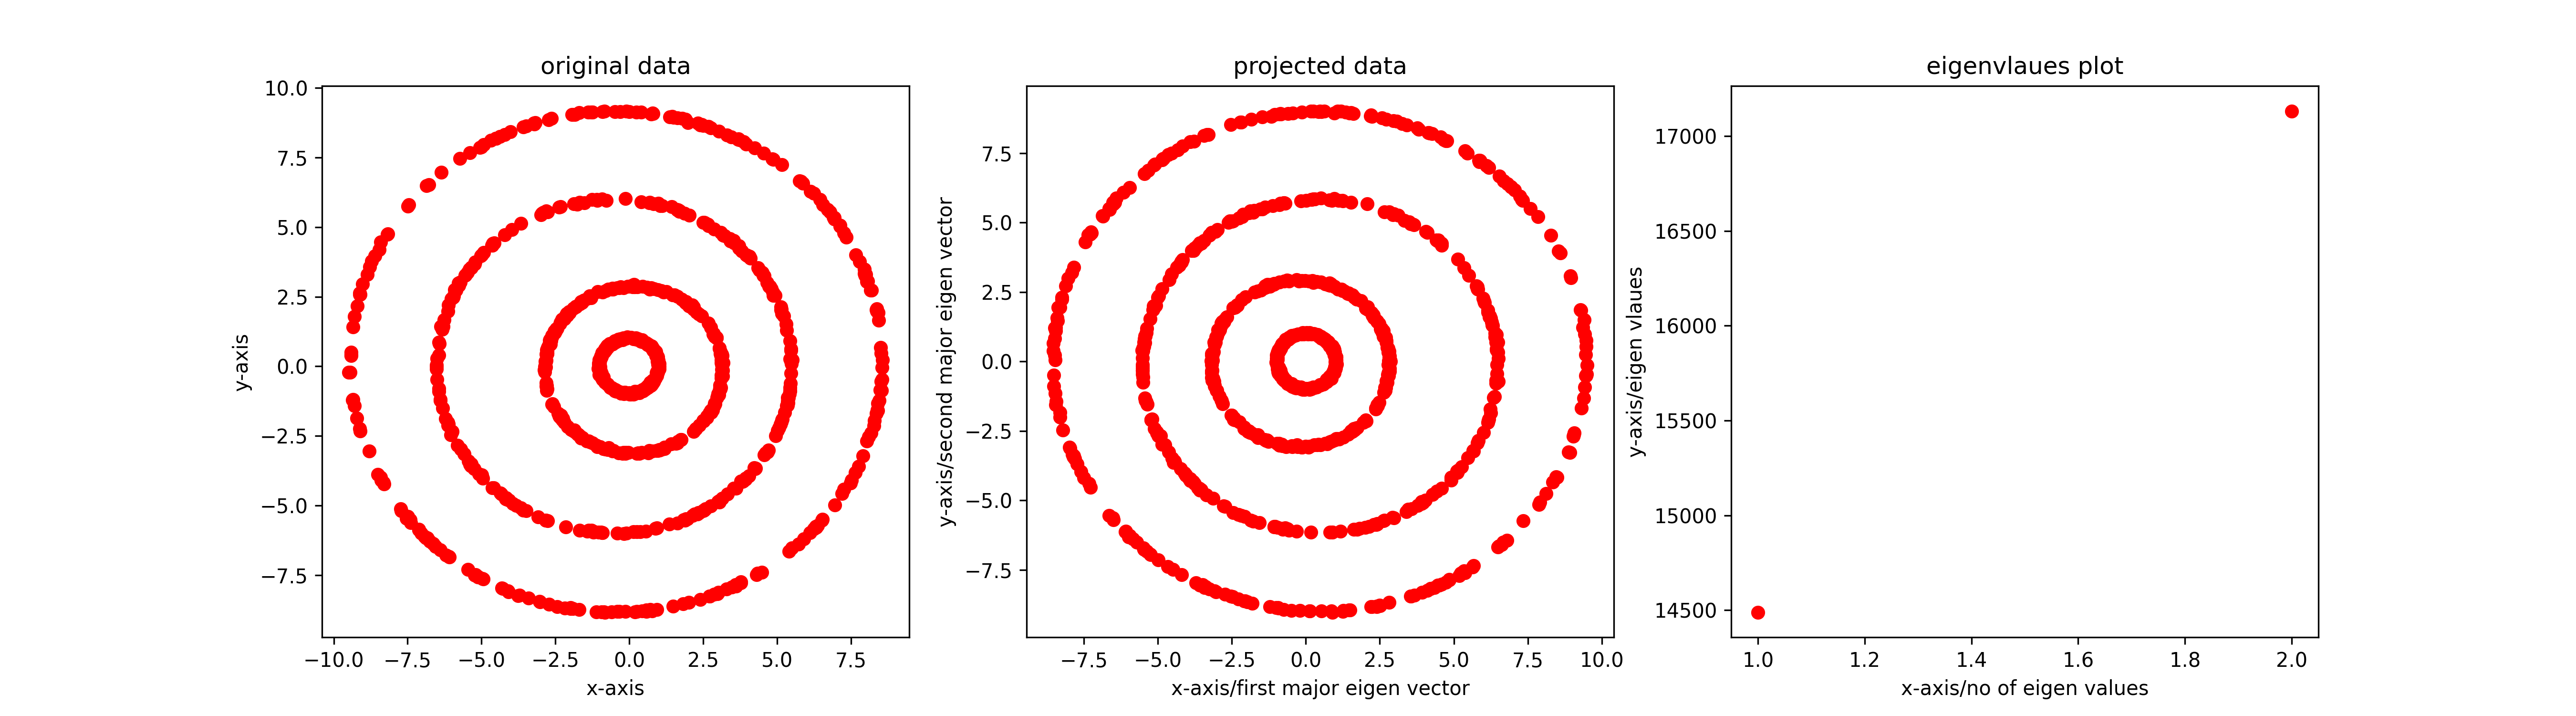
\includegraphics[width=15cm,height=5cm]{A.png}
\textbf{Figure1 :}  Result of centered data\\

Below figure shows the results for non-centered data	

\hangindent=5.5cm 
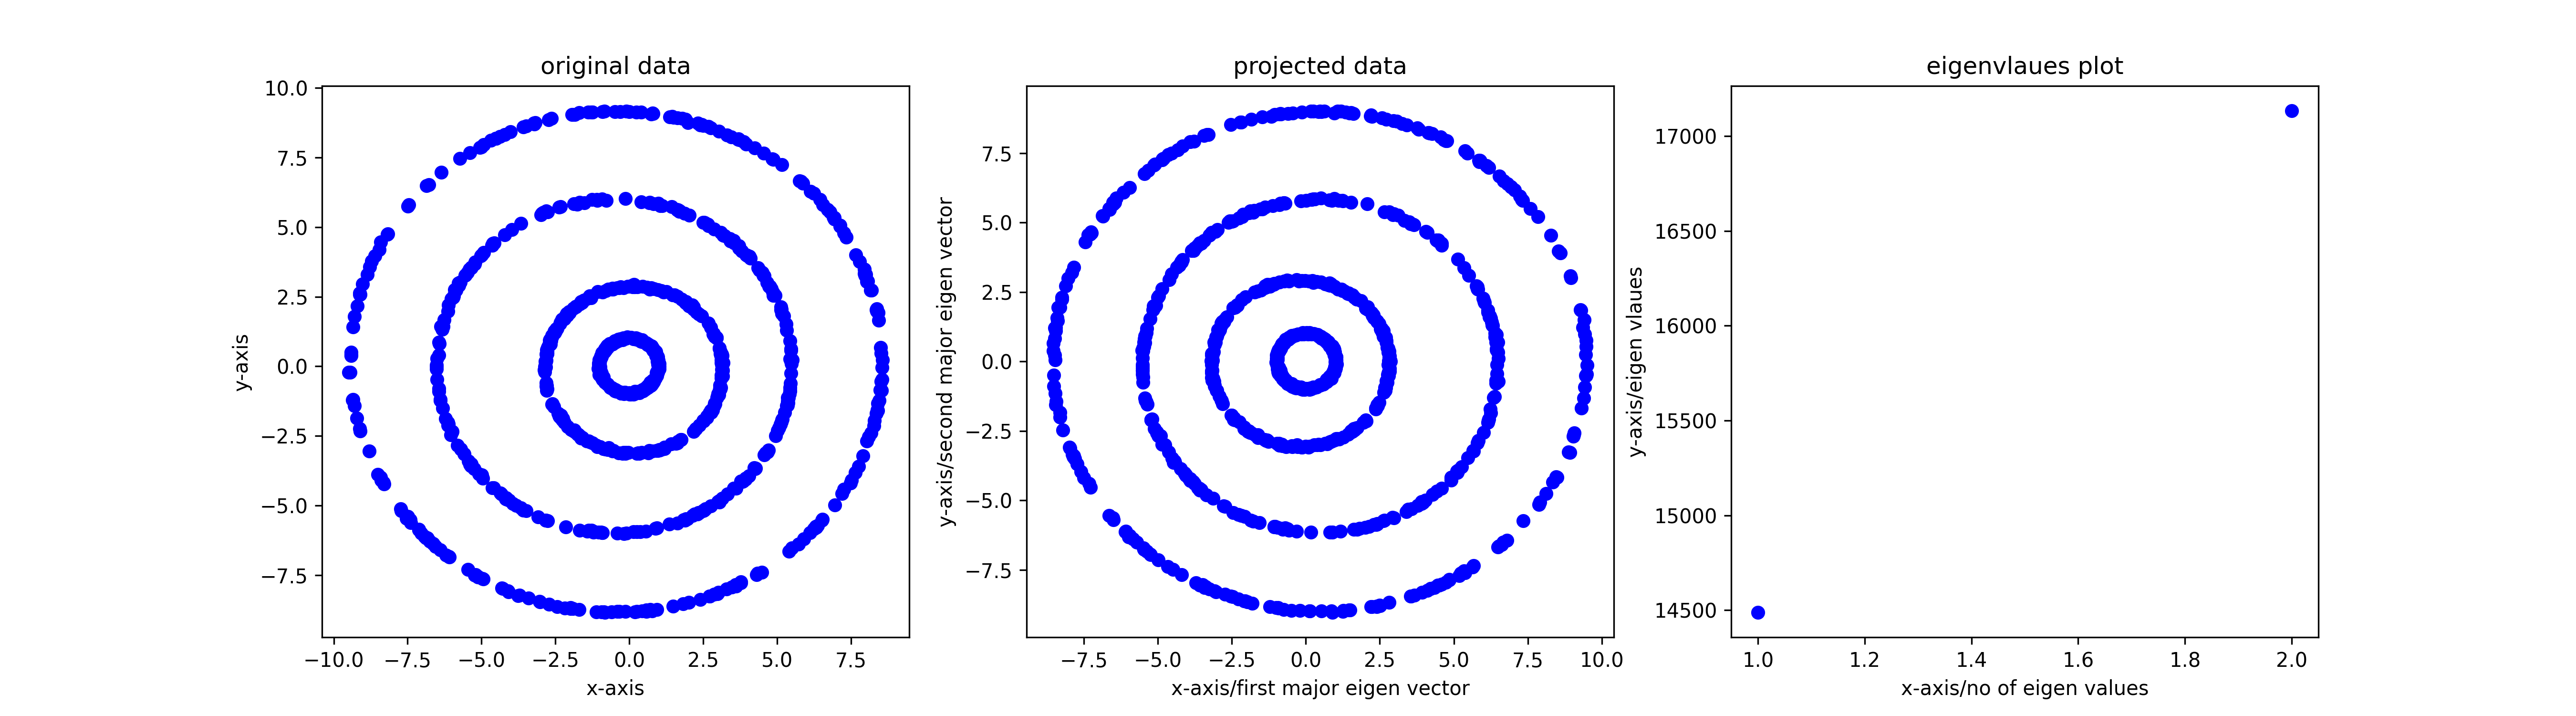
\includegraphics[width=15cm,height=5cm]{cA.png}
\textbf{Figure2 :}  Result of non centered data\\

\hangindent=0.0cm 
As the given data is already centered so centering does not plays any role here.

From figure it is clear that PCA is not able to do any helpful transformation on data, because, after projecting data onto eigen space we are obtaining the same data.\\

Also we are having the initial total variance of given data = total variance of projected data. as the data is circular around the origin, any pair of perpendicular vectors can become principal components directions.\\

\end{solution}
\part Write a piece of code to implement the Kernel PCA algorithm on this dataset.
Use the following kernels :

A. $k(x,y) = (1+x^Ty)^d$ for d = {2,3}

B. $k(x,y)= exp \frac{-(x-y)^T(x-y)}{2\sigma^2}$ for $\sigma={0.1,0.2,....,1}$

Plot the projection of each point in the dataset onto the top-2 components for
each kernel. Use one plot for each kernel and in the case of (B), use a different
plot for each value of $\sigma$
\begin{solution}
\textbf{Plots for kernel $k(x,y) = (1+x^Ty)^d$ are shown below}\\ 

\hangindent=5.5cm 
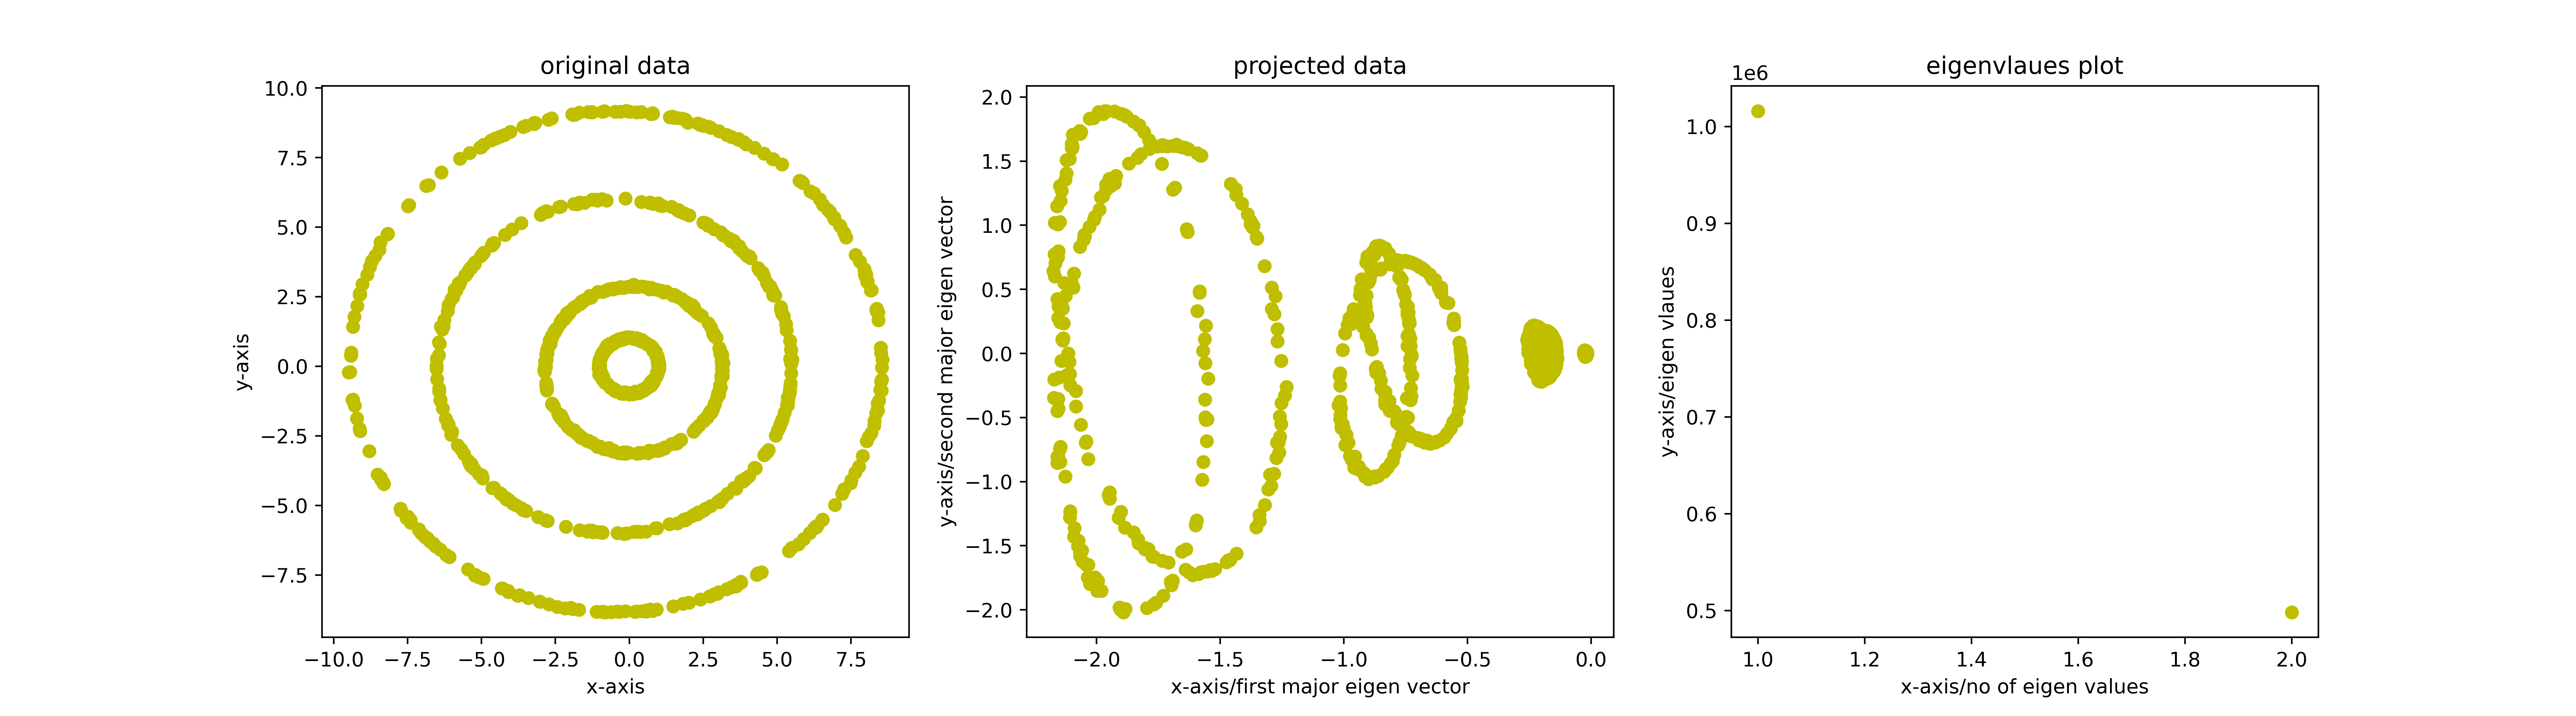
\includegraphics[width=15cm,height=5cm]{2.png}
\textbf{Figure 3 :} for d=2 \\

\hangindent=0.0cm 

\hangindent=5.5cm 
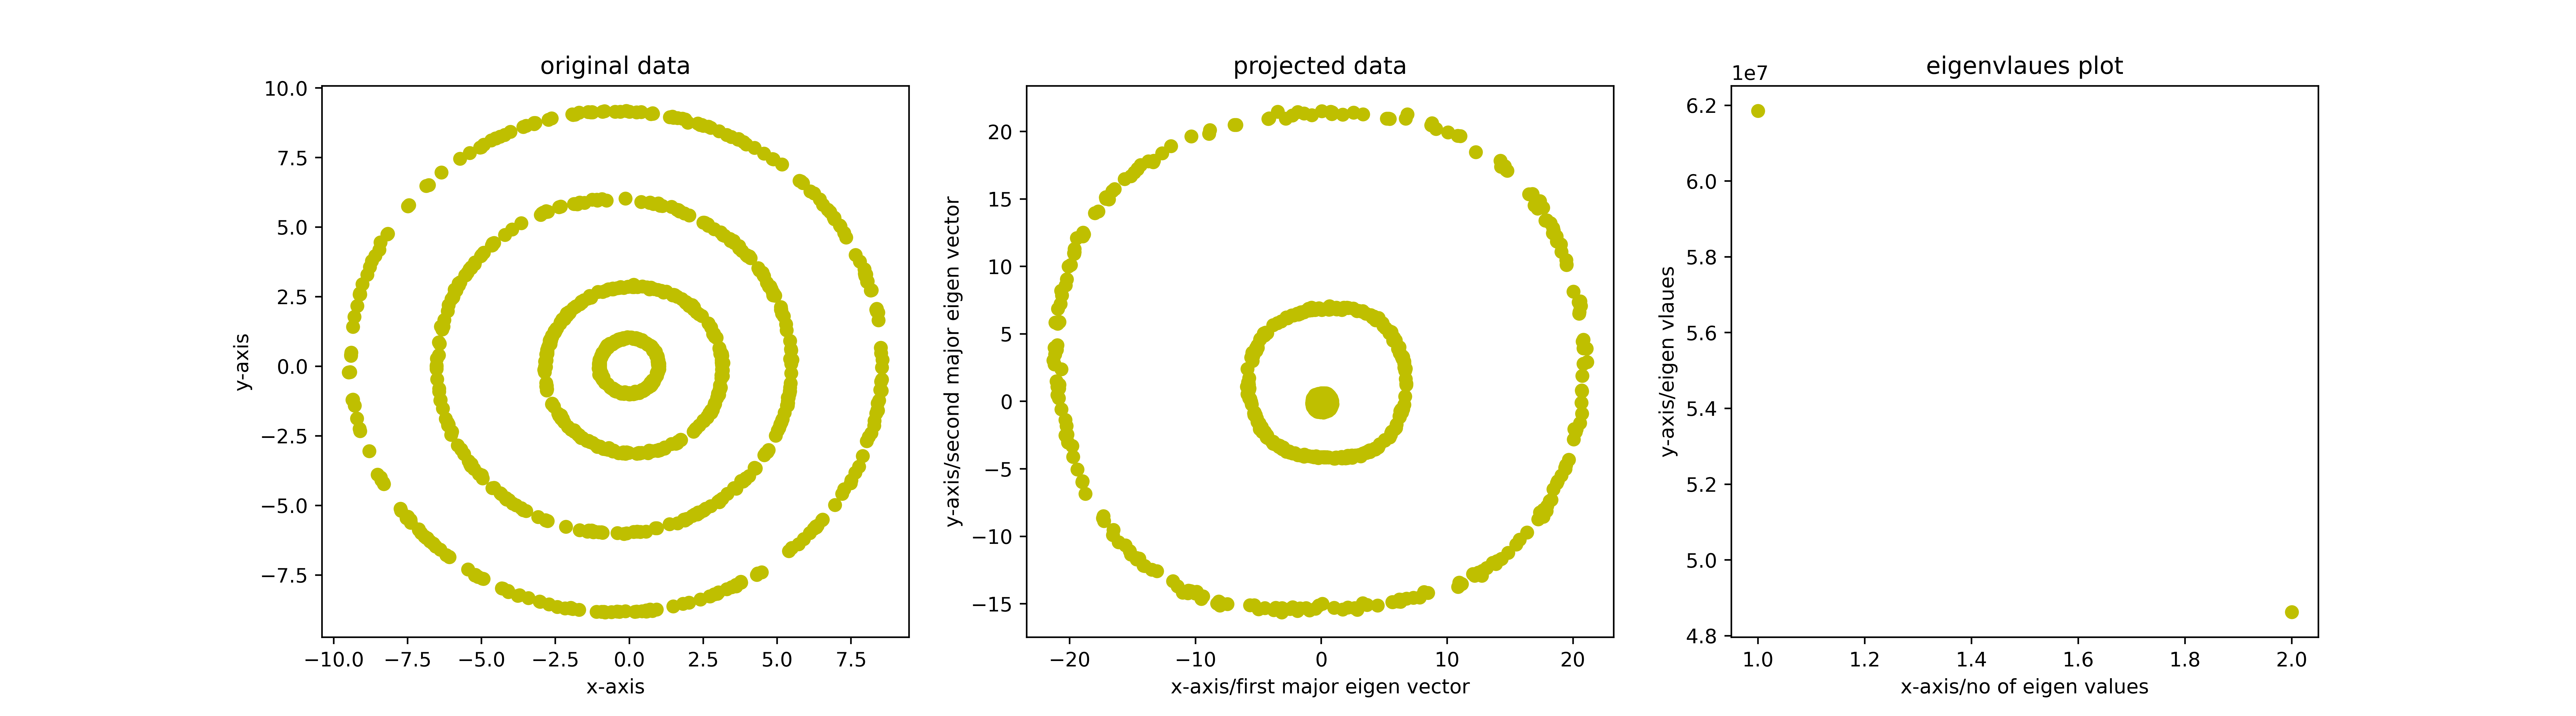
\includegraphics[width=15cm,height=5cm]{3.png}
\textbf{Figure 4 :} for d=3 \\

\hangindent=0.0cm 

\textbf{Plots for kernel $k(x,y) = (1+x^Ty)^d$ are shown below}\\ 

\hangindent=5.5cm 
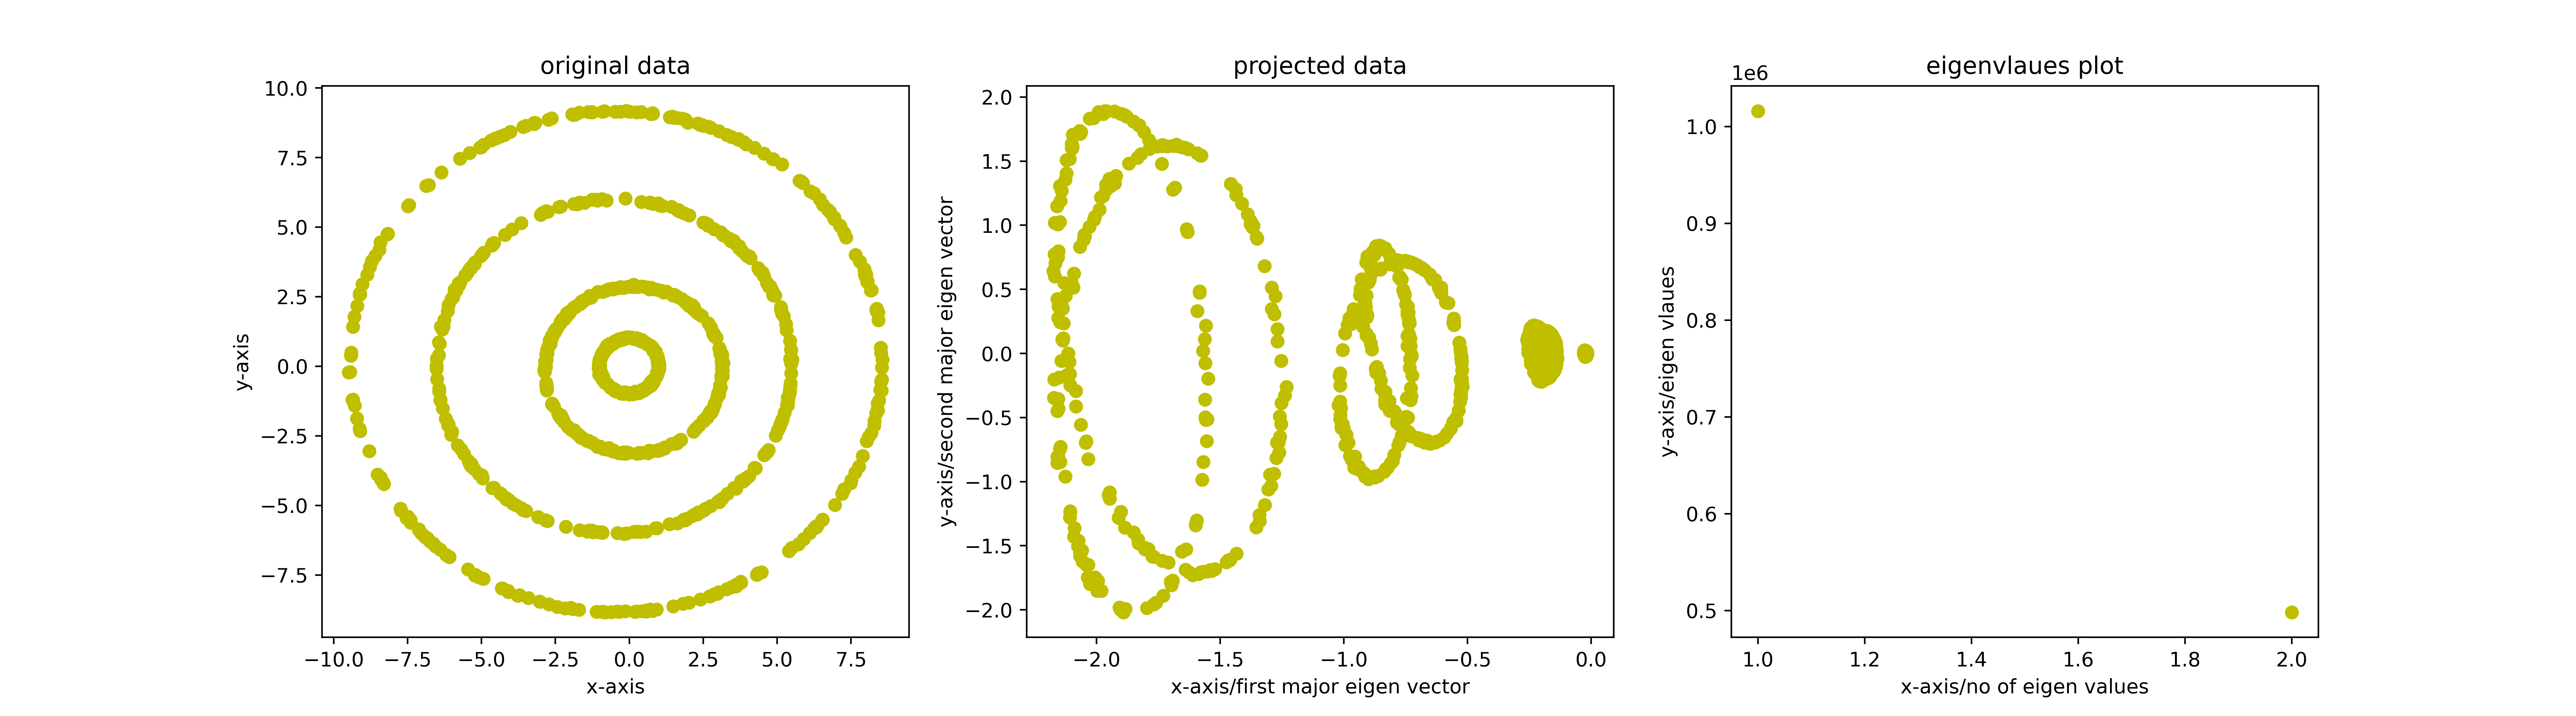
\includegraphics[width=15cm,height=5cm]{2.png}
\textbf{Figure 5:} for $\alpha$=0.1\\

\hangindent=0.0cm 

\hangindent=5.5cm 
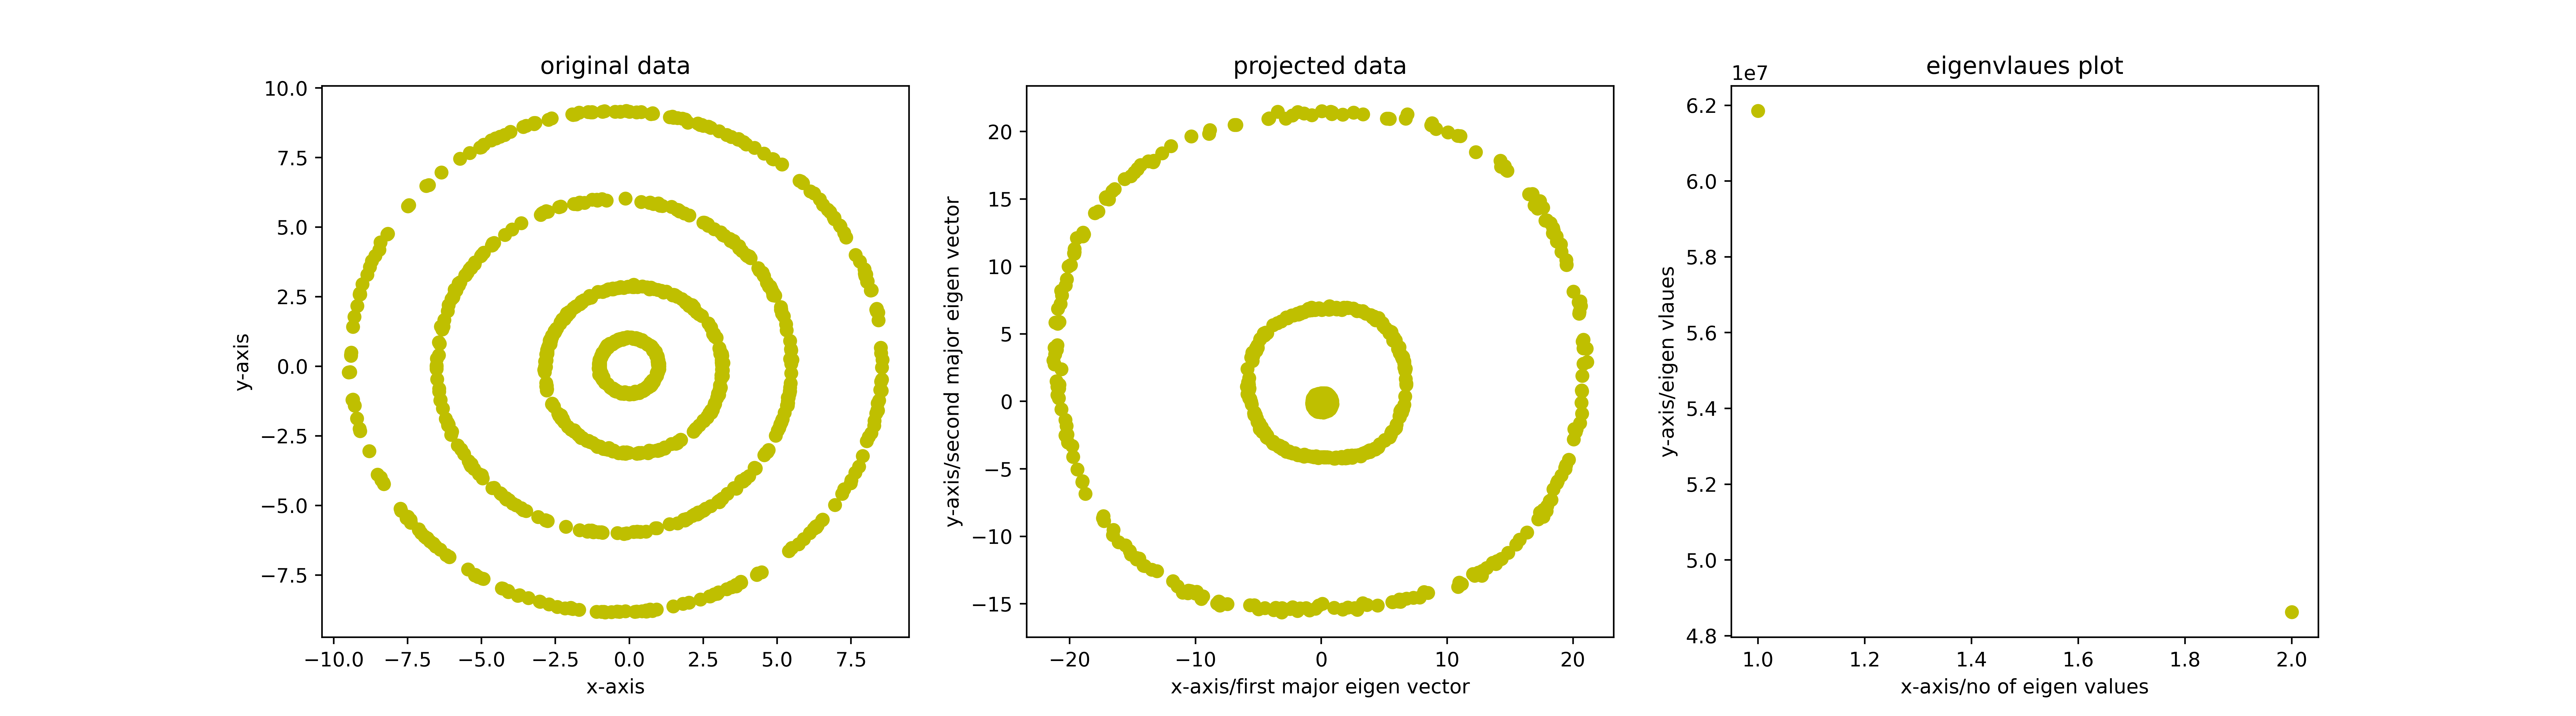
\includegraphics[width=15cm,height=5cm]{3.png}
\textbf{Figure 6 :} for $\alpha$=0.2 \\

\hangindent=0.0cm 

\hangindent=5.5cm 
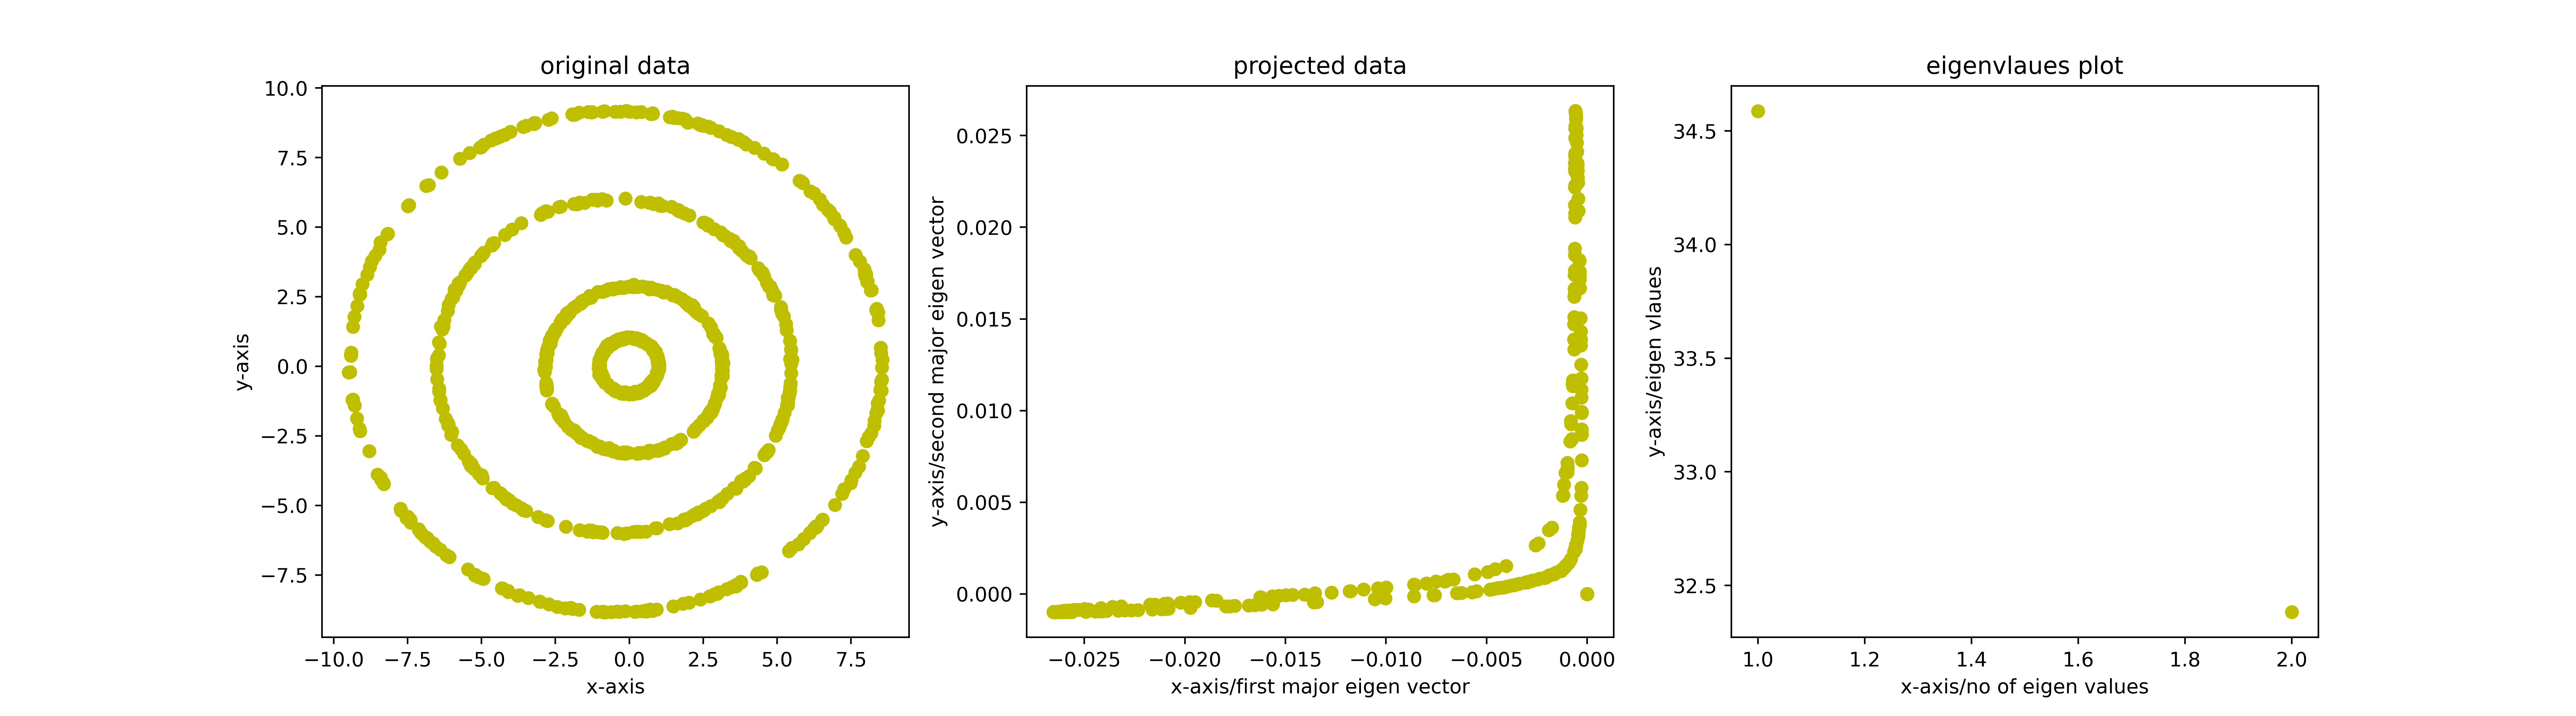
\includegraphics[width=15cm,height=5cm]{3k2.png}
\textbf{Figure 7 :} for $\alpha$=0.3 \\

\hangindent=0.0cm 

\hangindent=5.5cm 
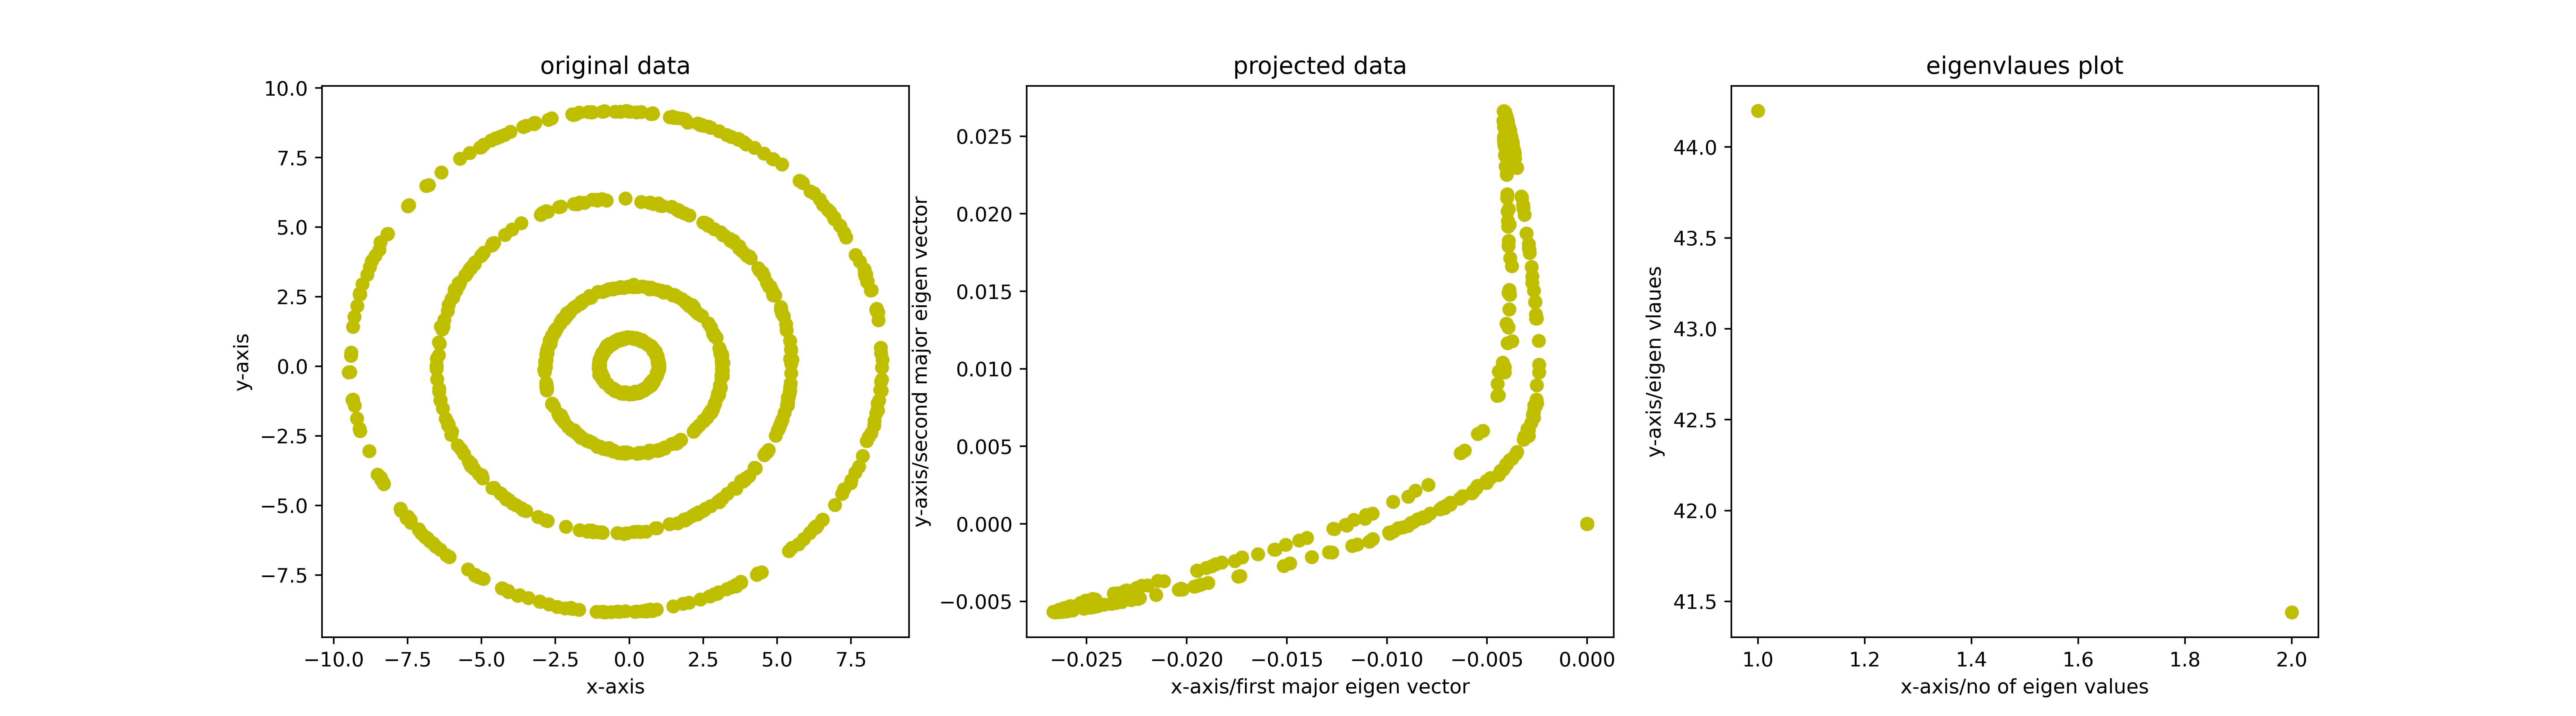
\includegraphics[width=15cm,height=5cm]{4k2.png}
\textbf{Figure 8 :} for $\alpha$=0.4 \\

\hangindent=0.0cm 

\hangindent=5.5cm 
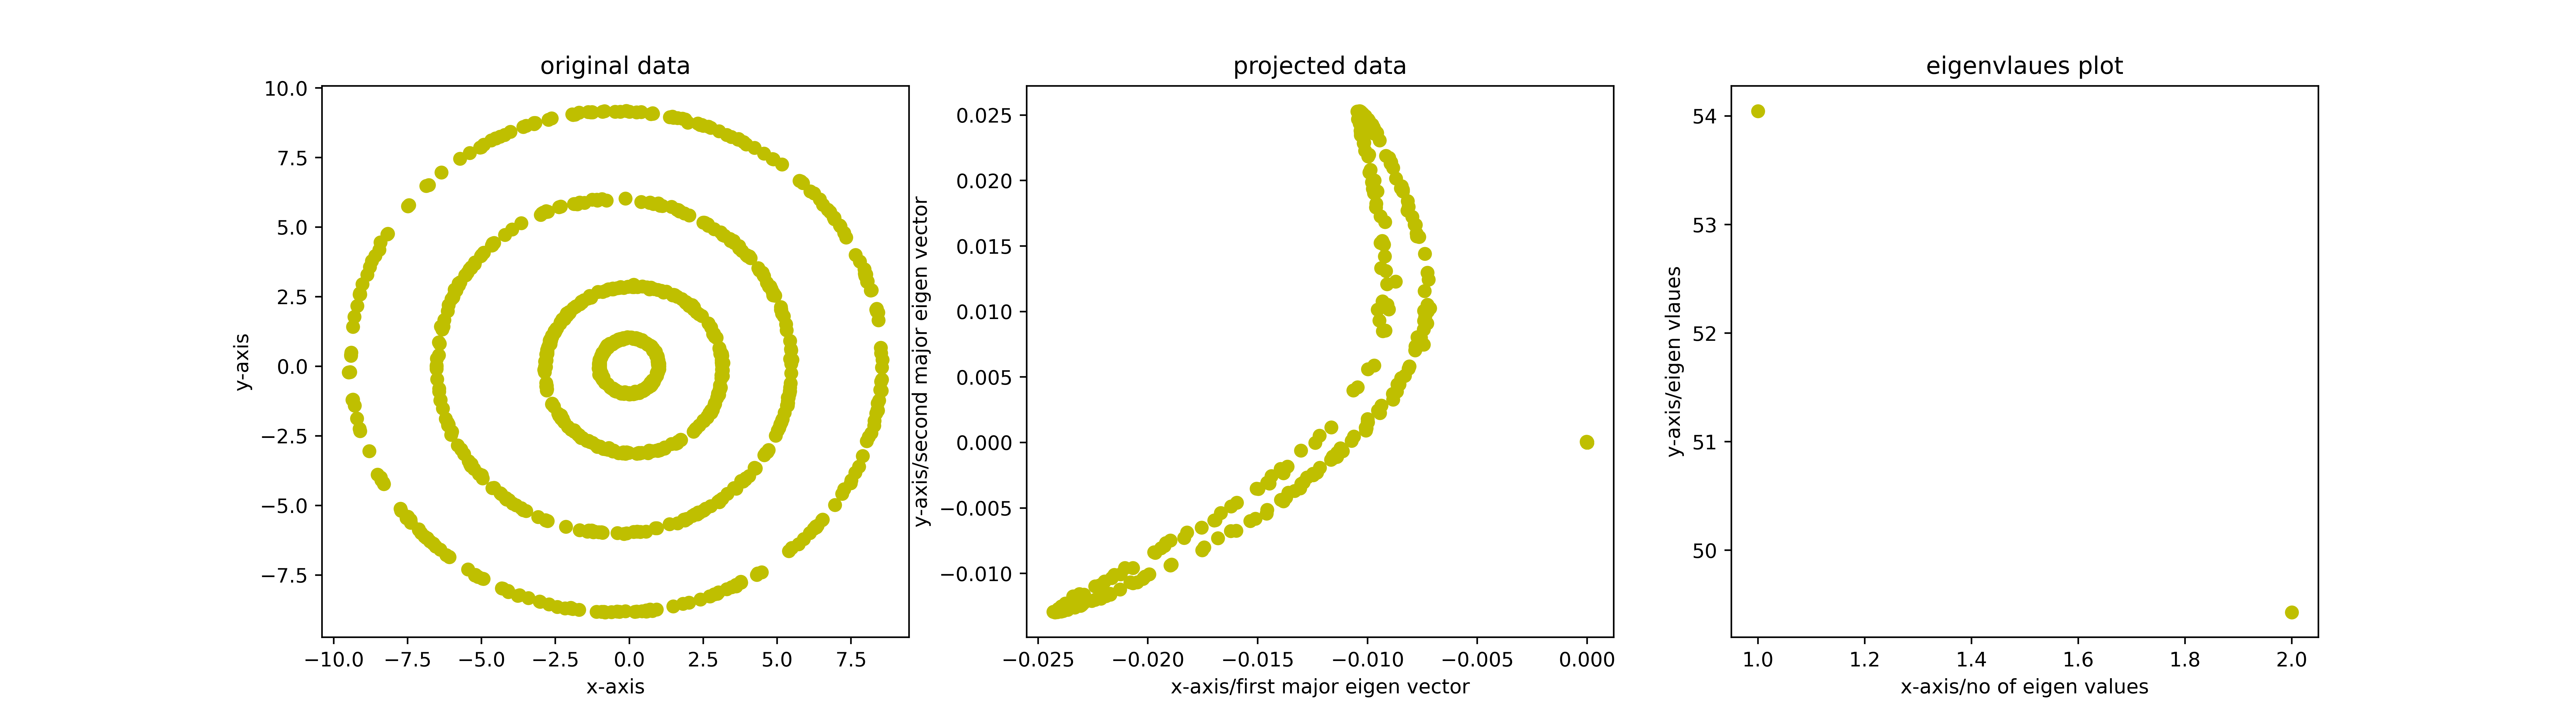
\includegraphics[width=15cm,height=5cm]{5k2.png}
\textbf{Figure 9 :} for $\alpha$=0.5 \\

\hangindent=0.0cm 
 
\hangindent=5.5cm 
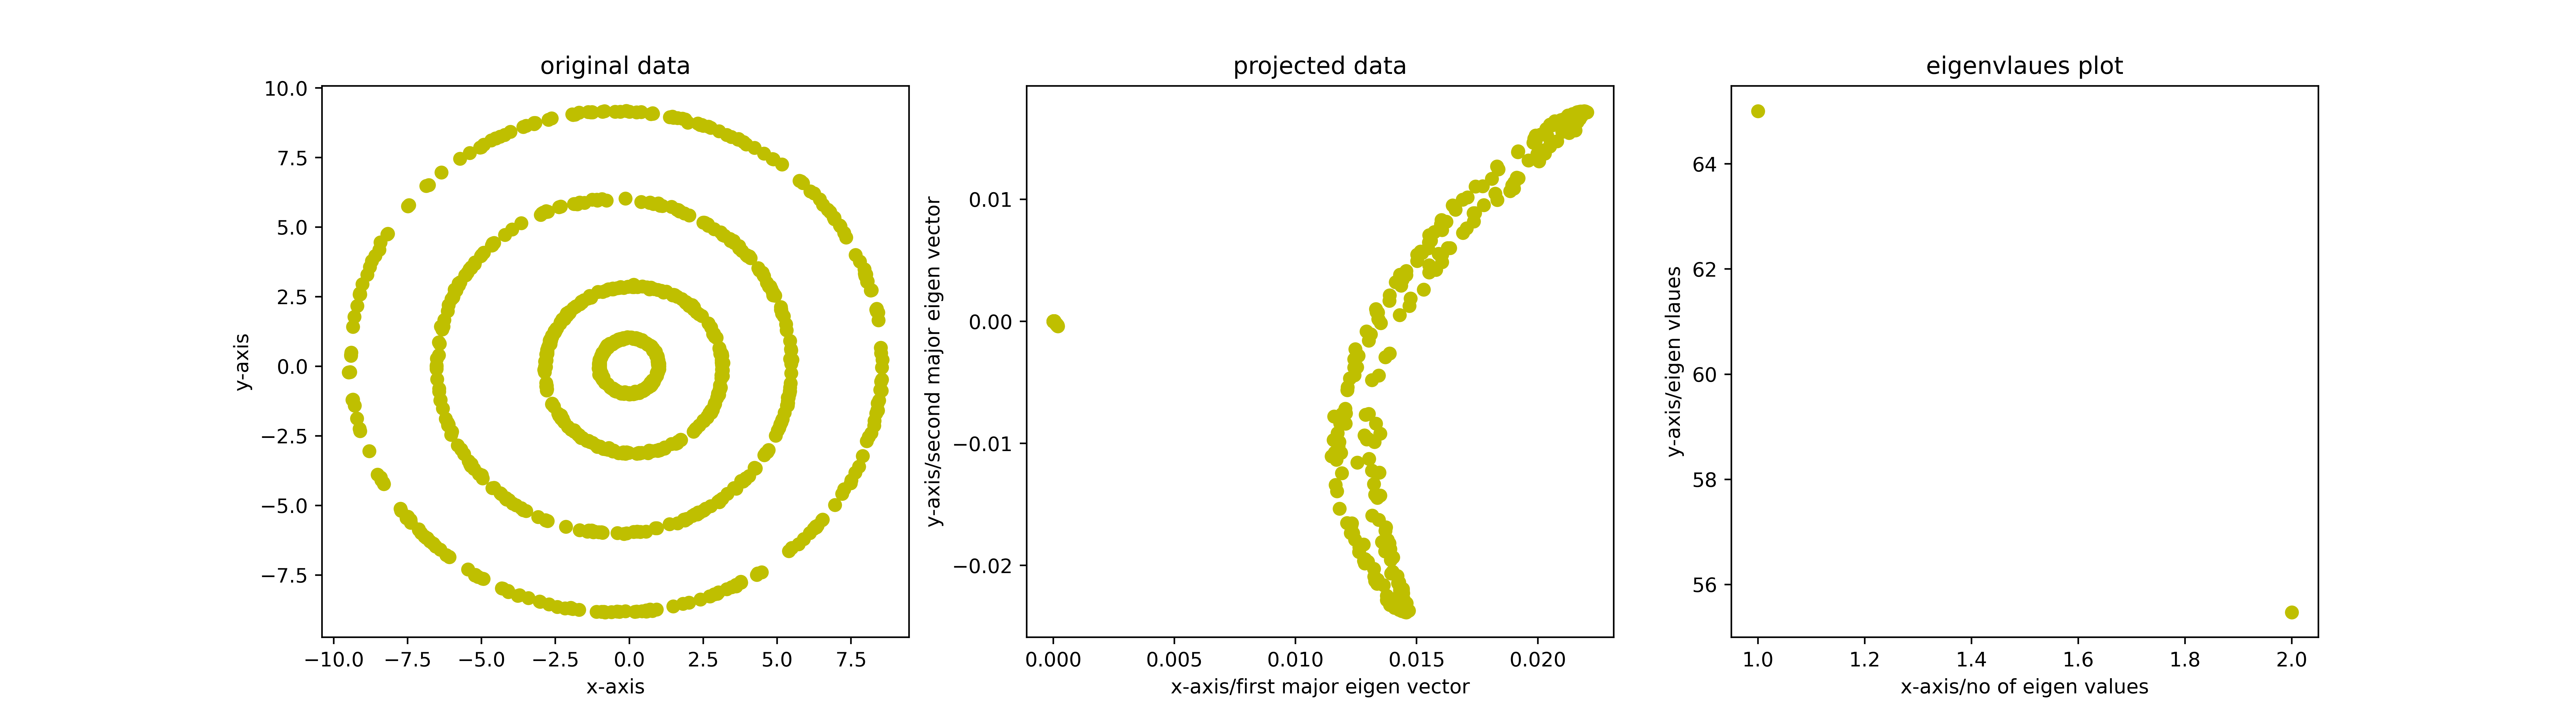
\includegraphics[width=15cm,height=5cm]{6k2.png}
\textbf{Figure 10 :} for $\alpha$=0.6 \\

\hangindent=0.0cm 

\hangindent=5.5cm 
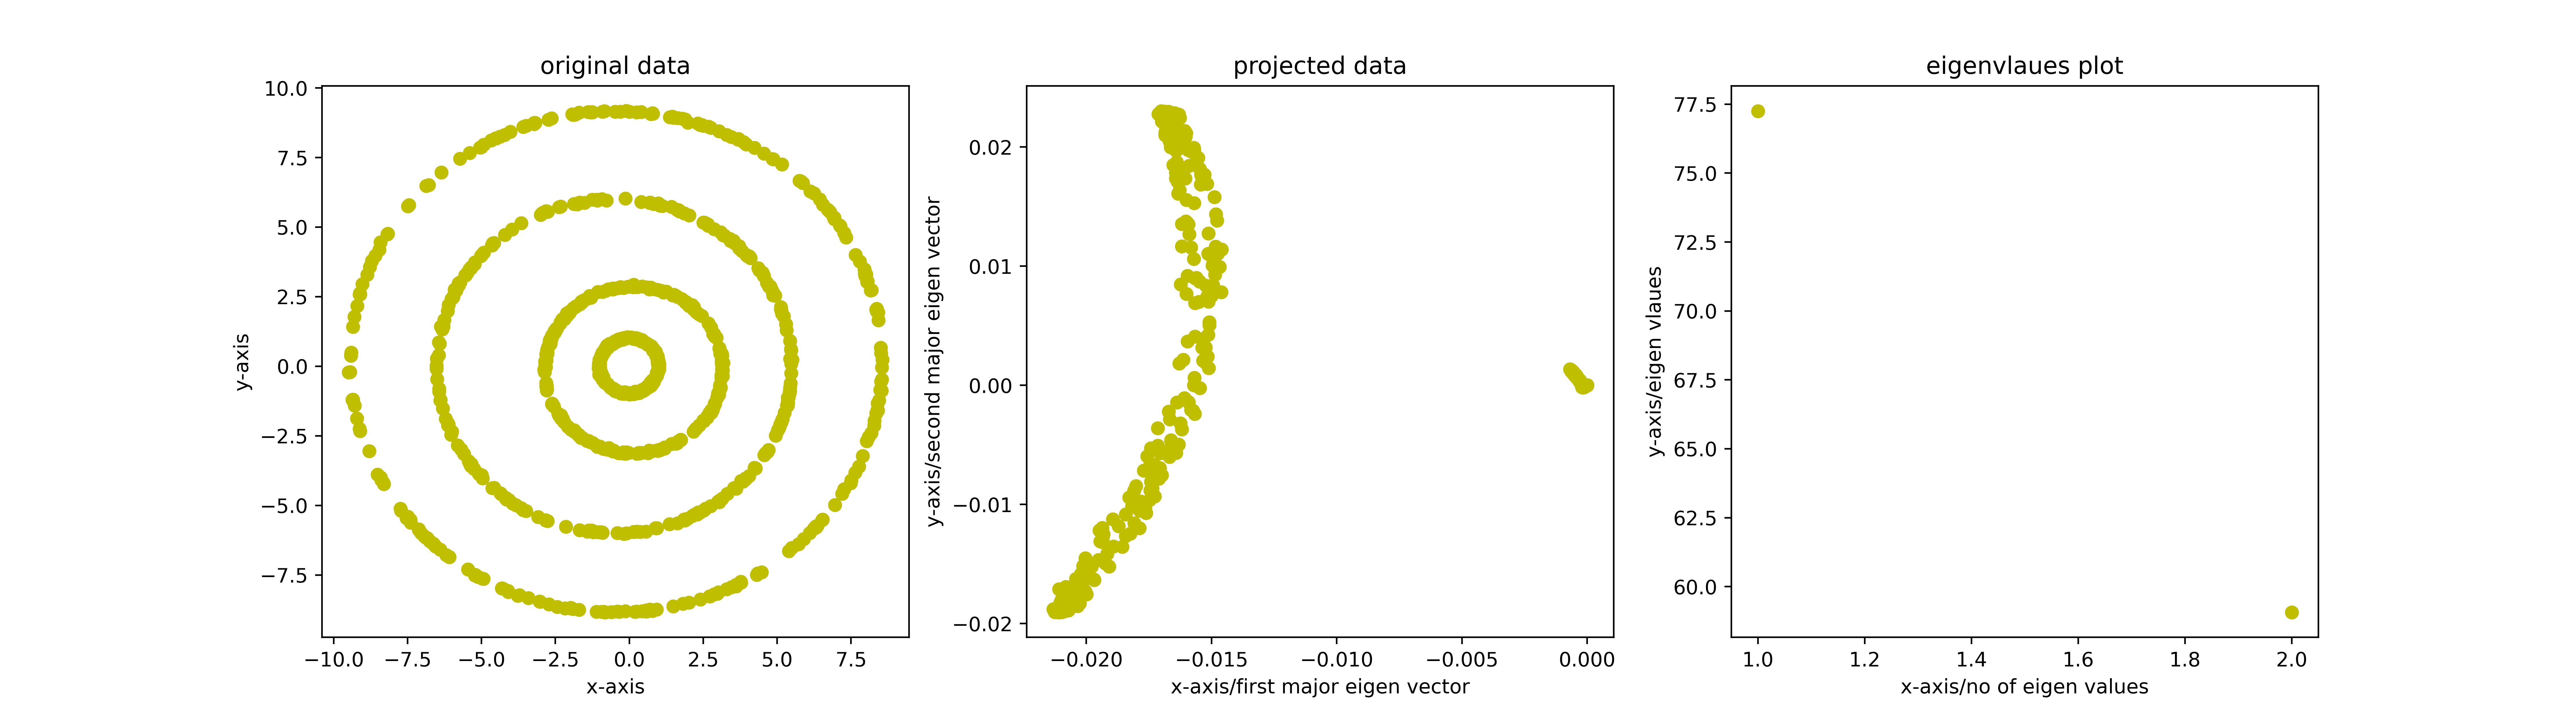
\includegraphics[width=15cm,height=5cm]{7k2.png}
\textbf{Figure 11 :} for $\alpha$=0.7 \\

\hangindent=0.0cm 

\hangindent=5.5cm 
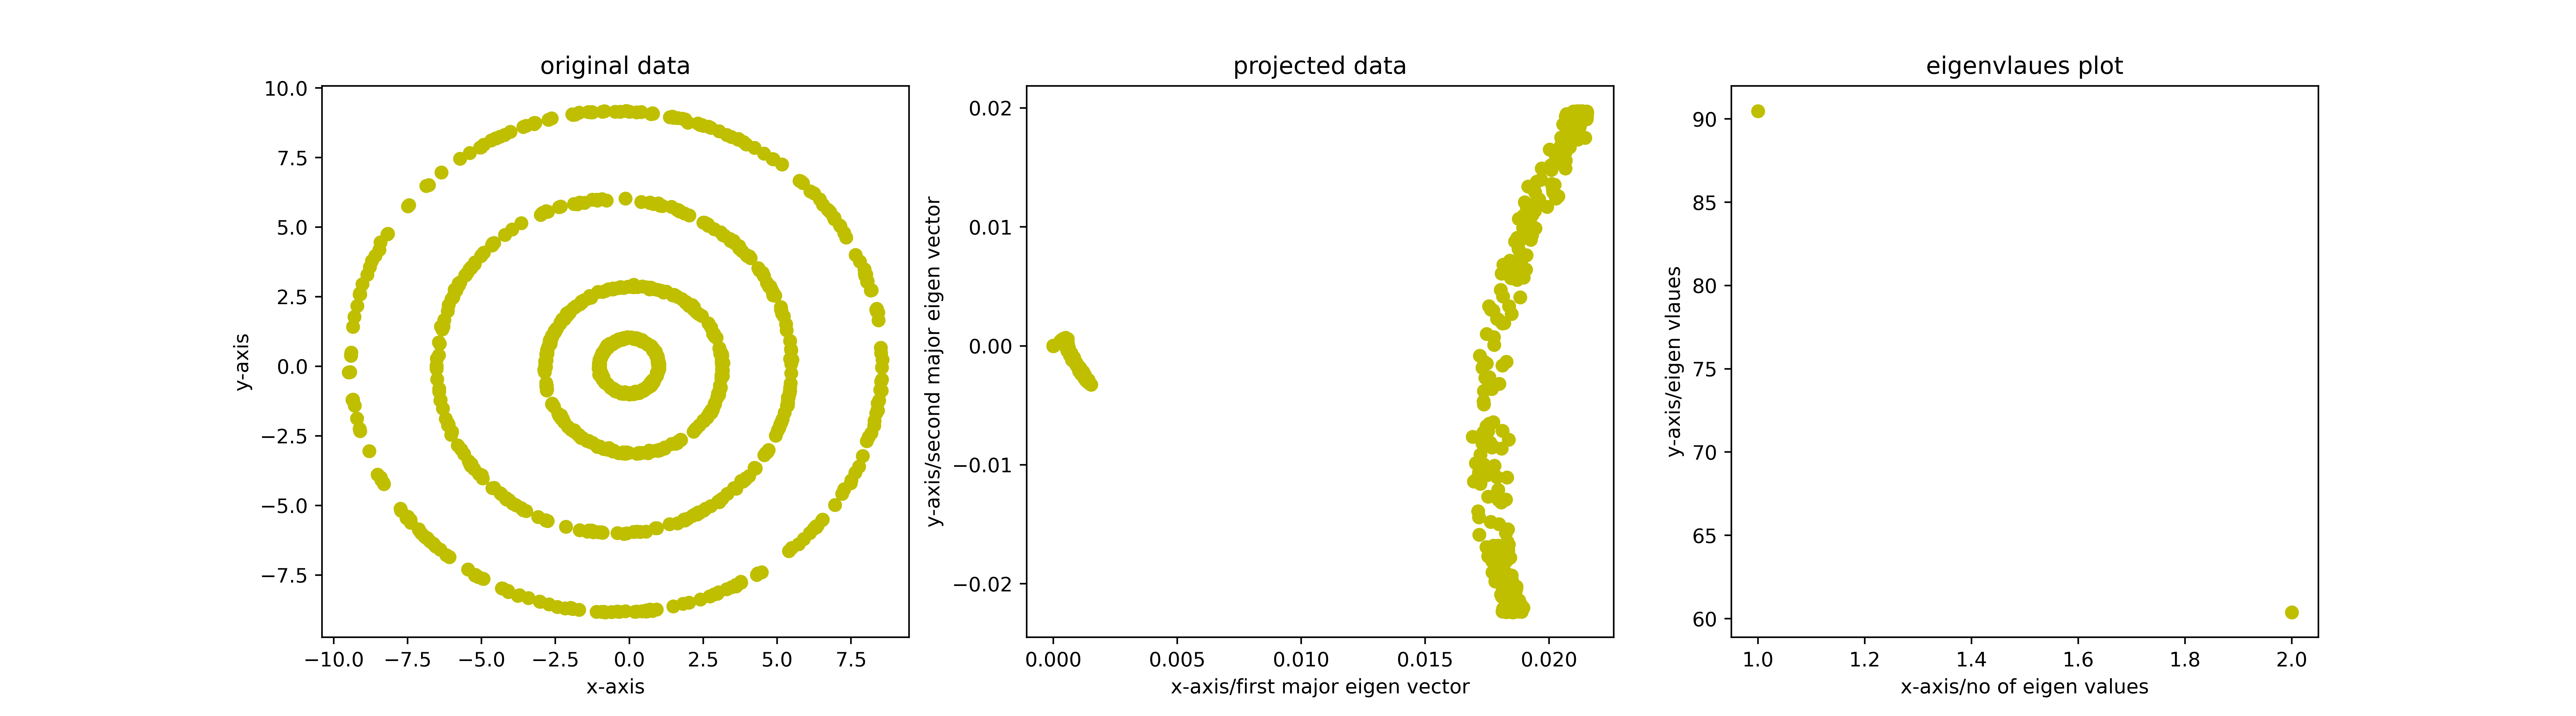
\includegraphics[width=15cm,height=5cm]{8k2.png}
\textbf{Figure 12 :} for $\alpha$=0.8 \\

\hangindent=0.0cm 

\hangindent=5.5cm 
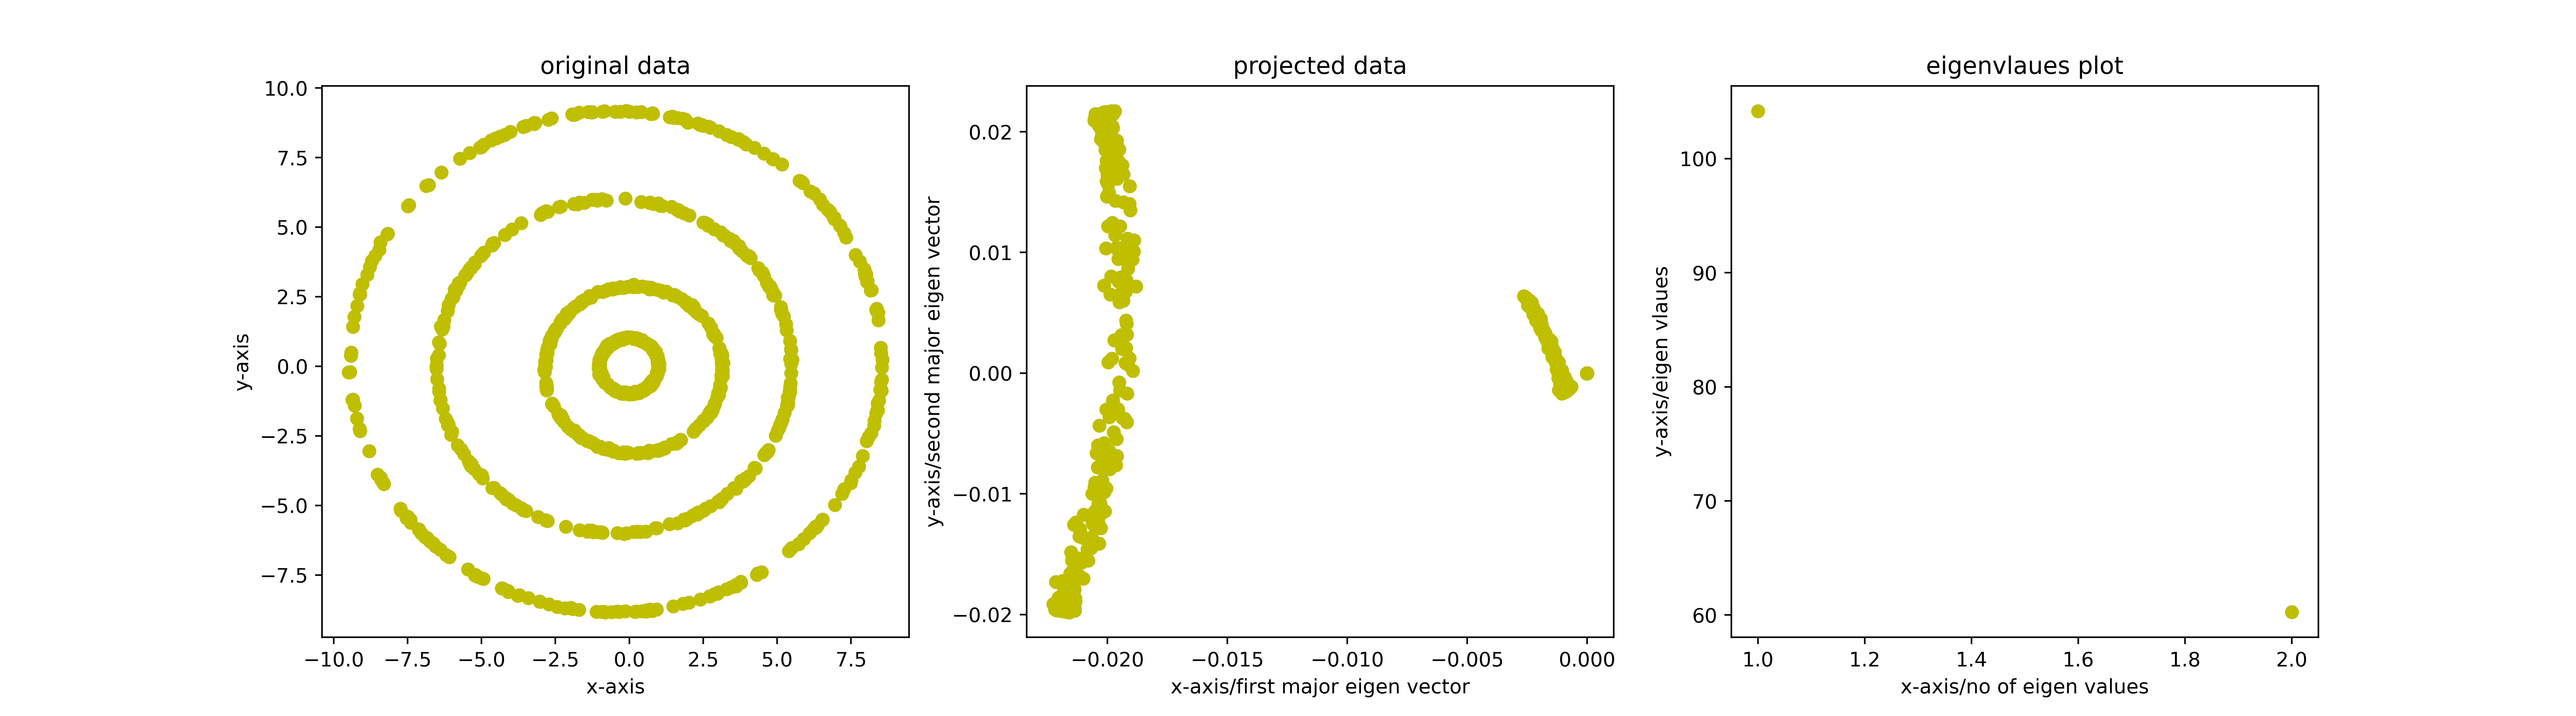
\includegraphics[width=15cm,height=5cm]{9k2.png}
\textbf{Figure 13 :} for $\alpha$=0.9 \\

\hangindent=0.0cm 

\hangindent=5.5cm 
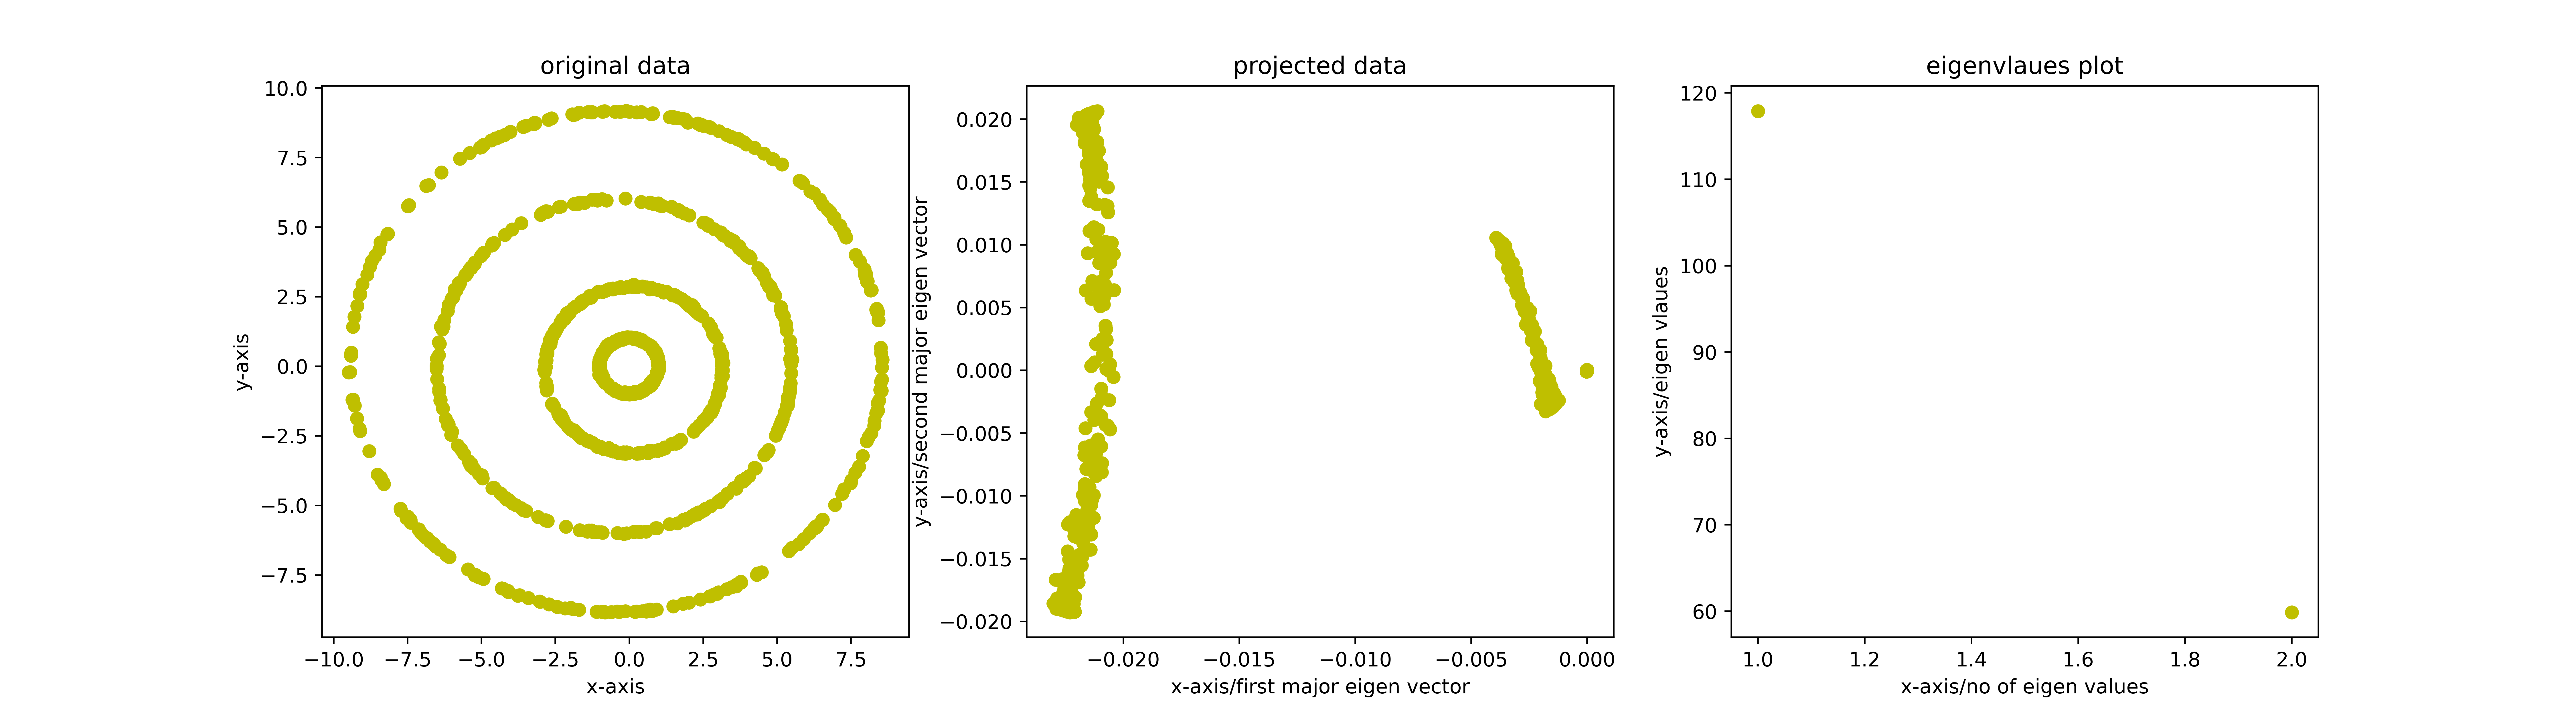
\includegraphics[width=15cm,height=5cm]{10k2.png}
\textbf{Figure 14 :} for $\alpha$=1.0 \\

\hangindent=0.0cm 

\end{solution}
\part Which Kernel do you think is best suited for this dataset and why?
\begin{solution} The gaussian kernel is best suited for this dataset with σ as 1,because it is capturing maximum variance among all other values of σ. The polynomial kernel is not able to properly de-correlate the data; it can be seen from figure 3 and figure 4 as compared to the gaussian kernel.

\end{solution}

\end{parts}

\question .

\begin{parts}
\part Write a piece of code to run the algorithm studied in class for the K-means
problem with k = 4 . 5 different random initialization and plot the error
function w.r.t iterations in each case. In each case, plot the clusters obtained in
different colors.
\begin{solution}

\hangindent=5.5cm 
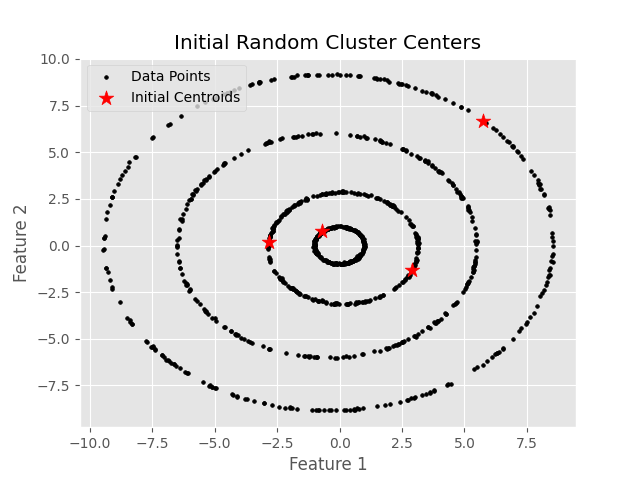
\includegraphics[width=.33\textwidth]{Q2a1_K4_1.png}\hfill
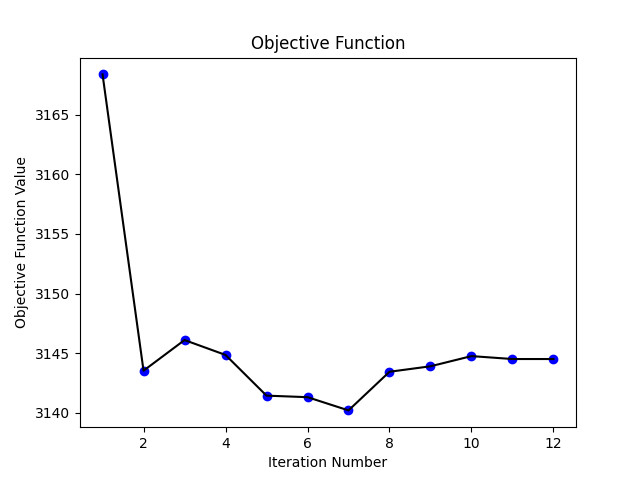
\includegraphics[width=.33\textwidth]{Q2a1_K4_2.png}\hfill
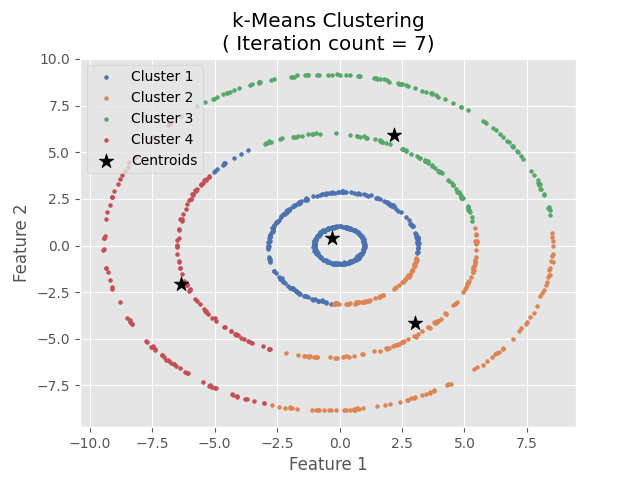
\includegraphics[width=.33\textwidth]{Q2a1_K4_3.png}
\textbf{Figure 15 :} Run 1 : no of clusters = 4\\

\hangindent=0.0cm 

\hangindent=5.5cm 
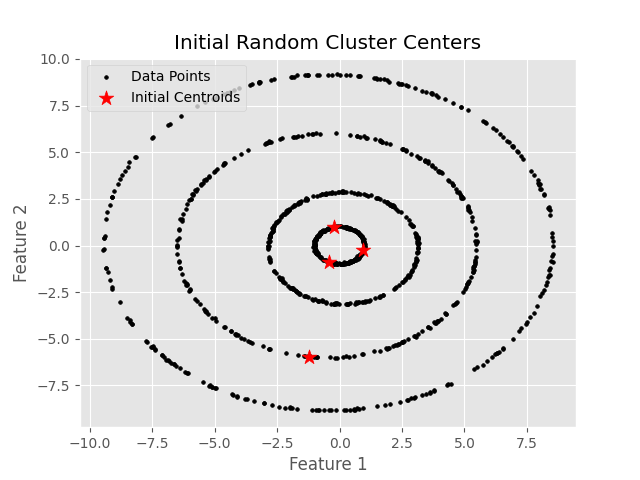
\includegraphics[width=.33\textwidth]{Q2a2_K4_1.png}\hfill
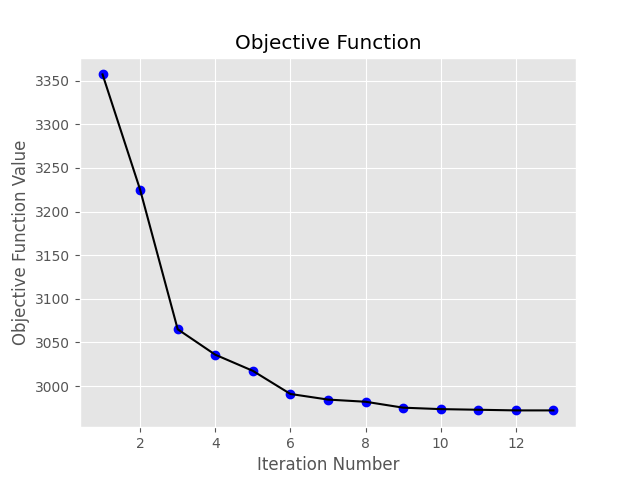
\includegraphics[width=.33\textwidth]{Q2a2_K4_2.png}\hfill
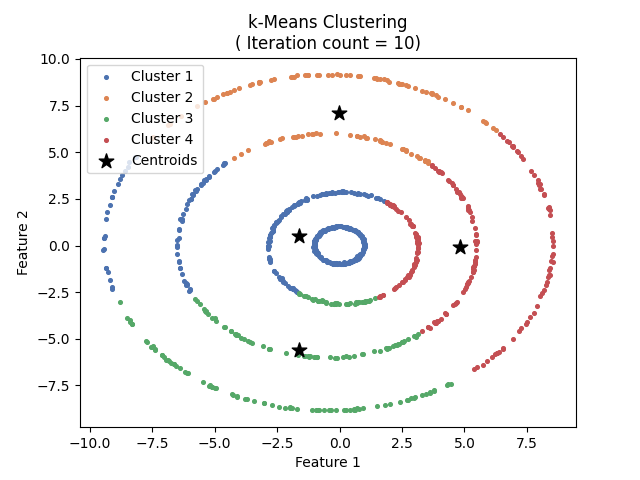
\includegraphics[width=.33\textwidth]{Q2a2_K4_3.png}
\textbf{Figure 16 :} Run 2 : no of clusters = 4\\

\hangindent=0.0cm 

\hangindent=5.5cm 
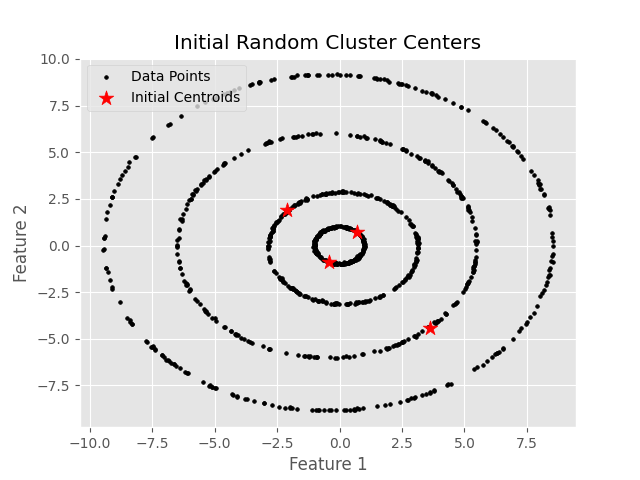
\includegraphics[width=.33\textwidth]{Q2a3_K4_1.png}\hfill
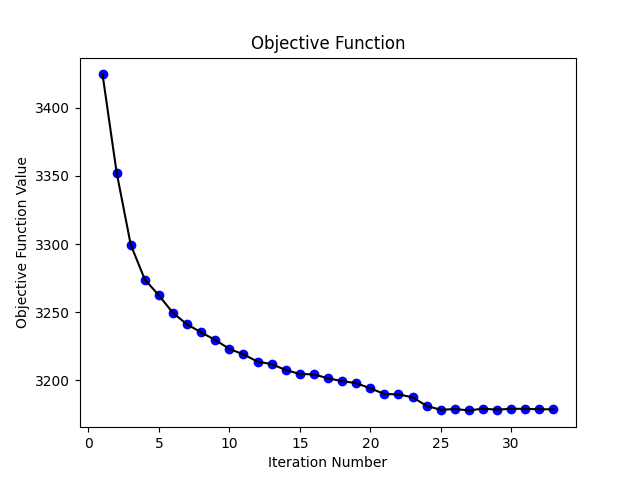
\includegraphics[width=.33\textwidth]{Q2a3_K4_2.png}\hfill
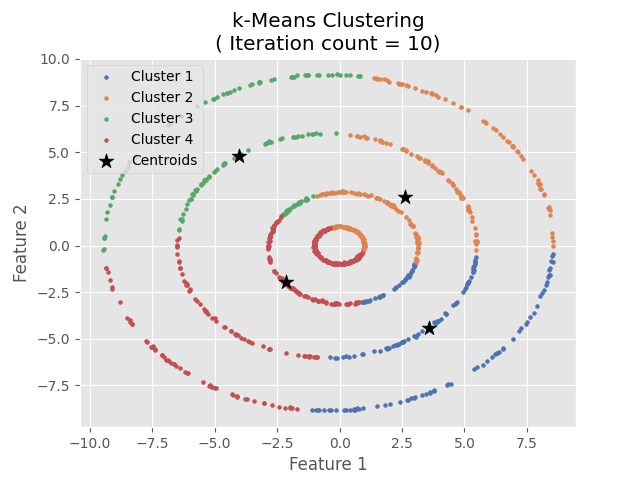
\includegraphics[width=.33\textwidth]{Q2a3_K4_3.png}
\textbf{Figure 17 :} Run 3 : no of clusters = 4\\

\hangindent=0.0cm 

\hangindent=5.5cm 
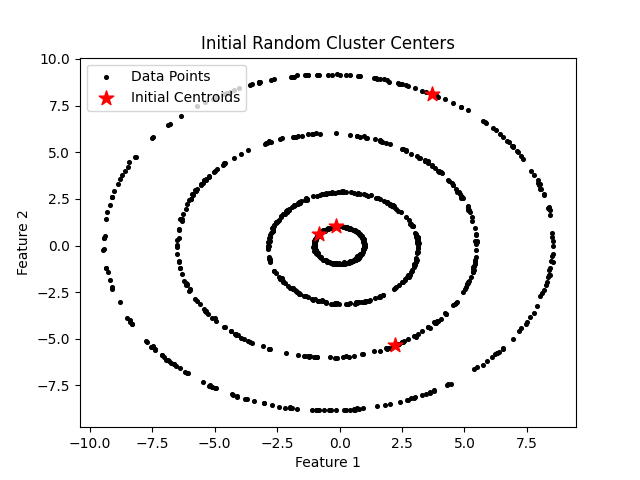
\includegraphics[width=.33\textwidth]{Q2a4_K4_1.png}\hfill
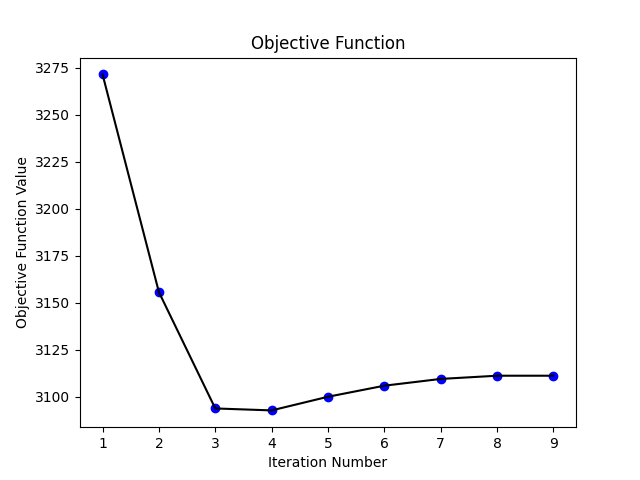
\includegraphics[width=.33\textwidth]{Q2a4_K4_2.png}\hfill
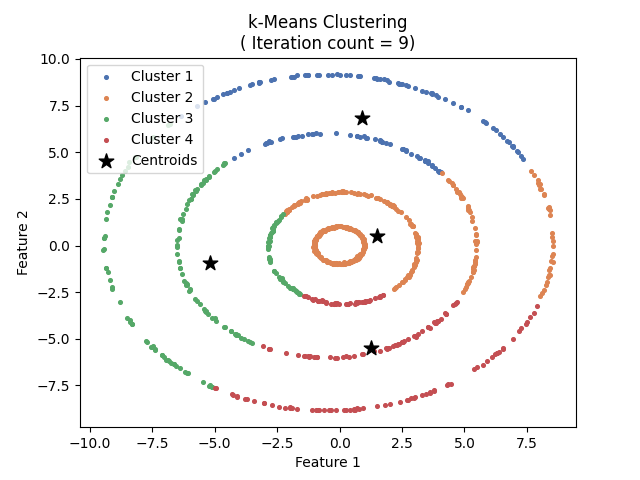
\includegraphics[width=.33\textwidth]{Q2a4_K4_3.png}
\textbf{Figure 17 :} Run 4 : no of clusters = 4\\

\hangindent=0.0cm 

\hangindent=5.5cm 
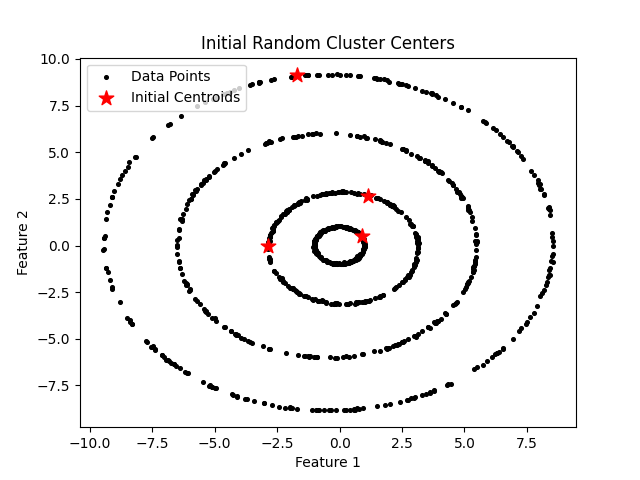
\includegraphics[width=.33\textwidth]{Q2a5_K4_1.png}\hfill
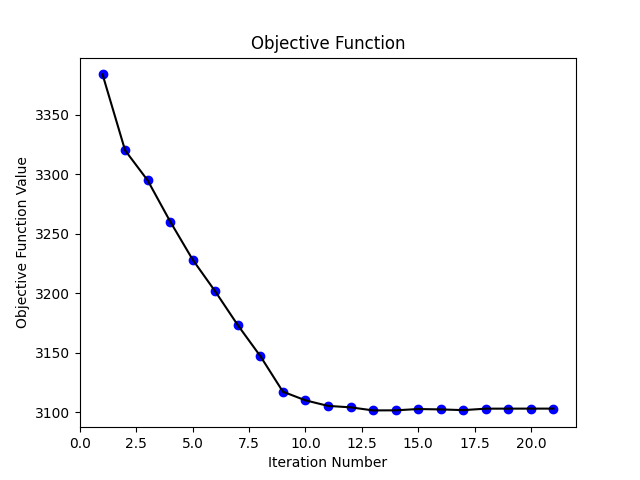
\includegraphics[width=.33\textwidth]{Q2a5_K4_2.png}\hfill
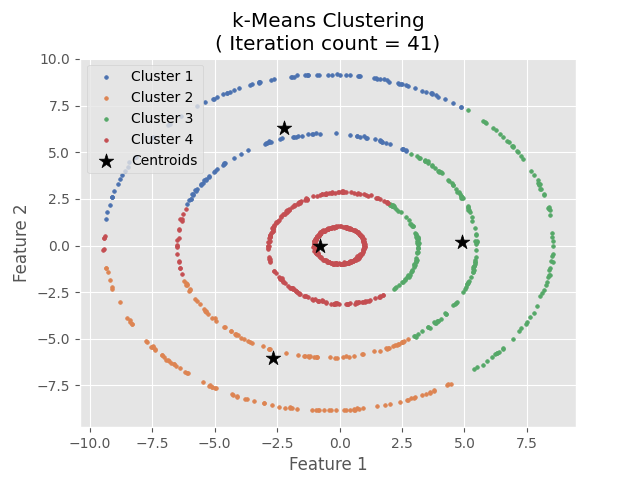
\includegraphics[width=.33\textwidth]{Q2a5_K4_3.png}
\textbf{Figure 17 :} Run  5: no of clusters = 4\\

\hangindent=0.0cm 

\end{solution}

\part Fix a random initialization. For $K = {2,3,4,5}$, obtain cluster centers according
to K-means algorithm using the fixed initialization. For each value of K, plot the
Voronoi regions associated to each cluster center. (You can assume the minimum
and maximum value in the data-set to be the range for each component of R2).\\
\begin{solution} Fixed a random initialization and  $K = {2,3,4,5}$,\\

\hangindent=5.5cm 
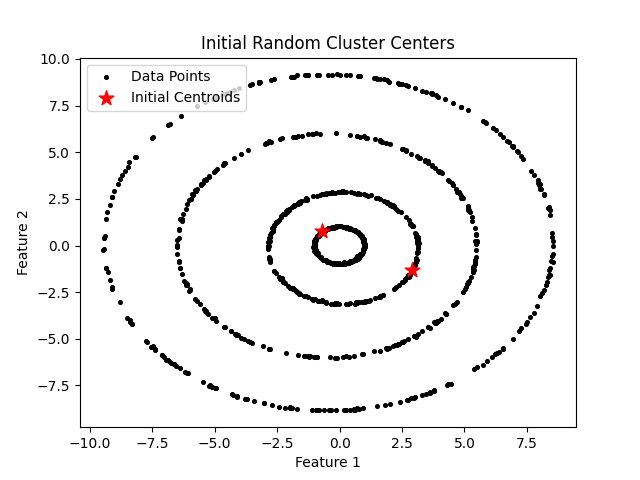
\includegraphics[width=.32\textwidth]{Q2b2_K4_1.png}\hfill
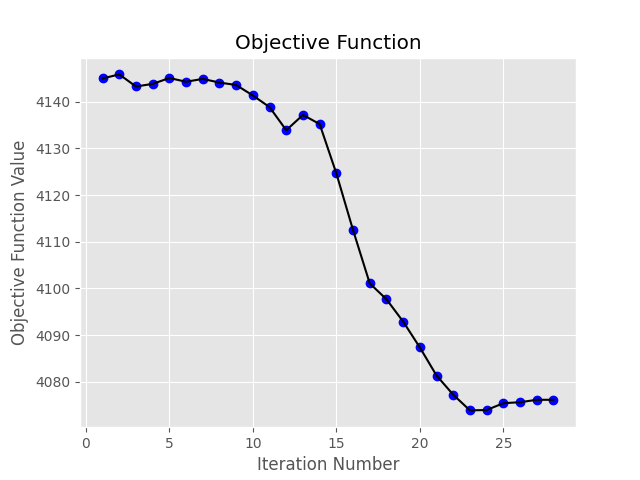
\includegraphics[width=.32\textwidth]{Q2b2_K4_2.png}\hfill
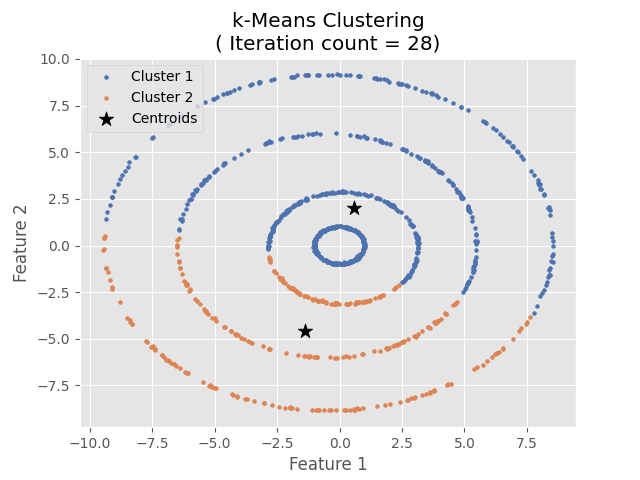
\includegraphics[width=.32\textwidth]{Q2b2_K4_3.png}
\textbf{Figure 18 :} Run  1: no of clusters = 2\\

\hangindent=0.0cm 

\hangindent=4.5cm 
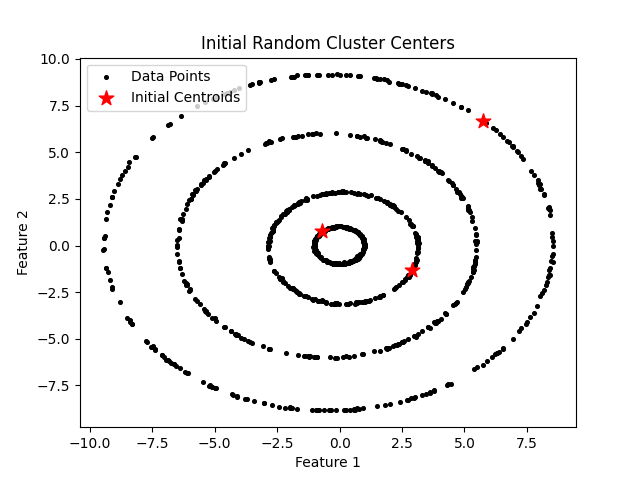
\includegraphics[width=.32\textwidth]{Q2b3_K4_1.png}\hfill
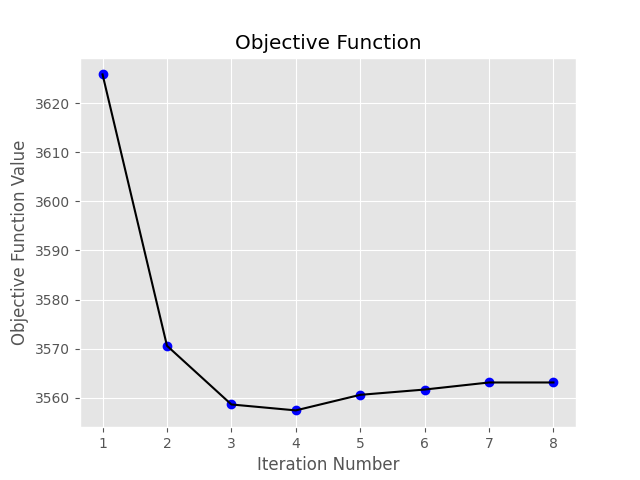
\includegraphics[width=.32\textwidth]{Q2b3_K4_2.png}\hfill
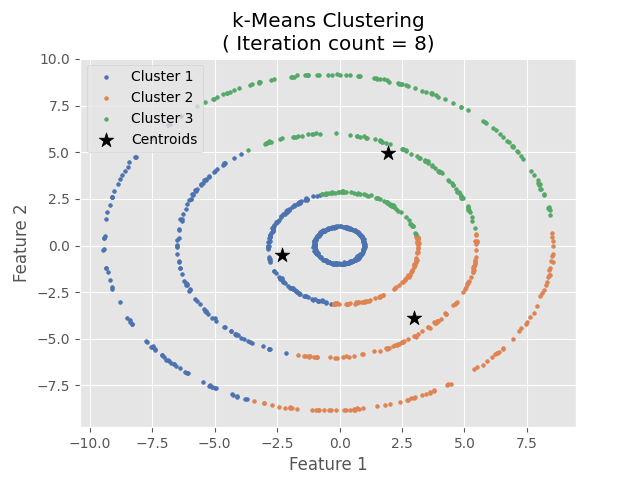
\includegraphics[width=.32\textwidth]{Q2b3_K4_3.png}
\textbf{Figure 18 :} Run 2: no of clusters = 3\\

\hangindent=0.0cm 

\hangindent=4.5cm 
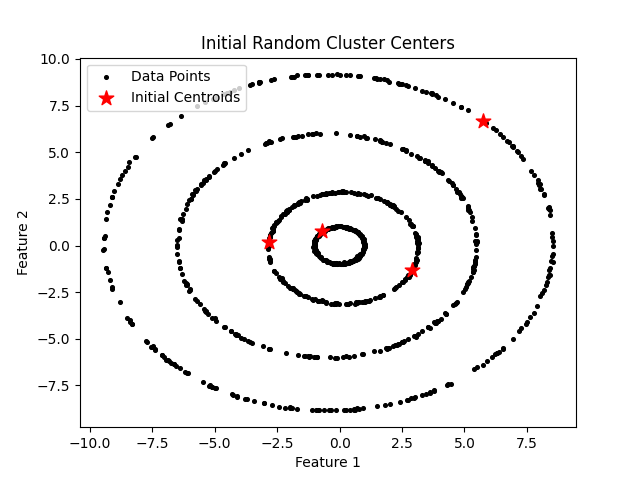
\includegraphics[width=.32\textwidth]{Q2b4_K4_1.png}\hfill
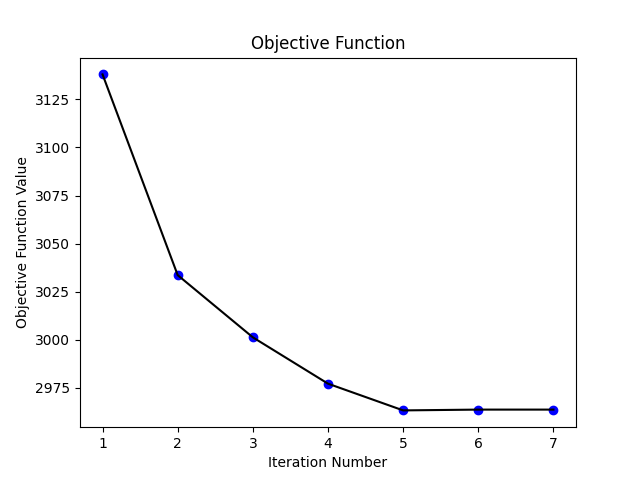
\includegraphics[width=.32\textwidth]{Q2b4_K4_2.png}\hfill
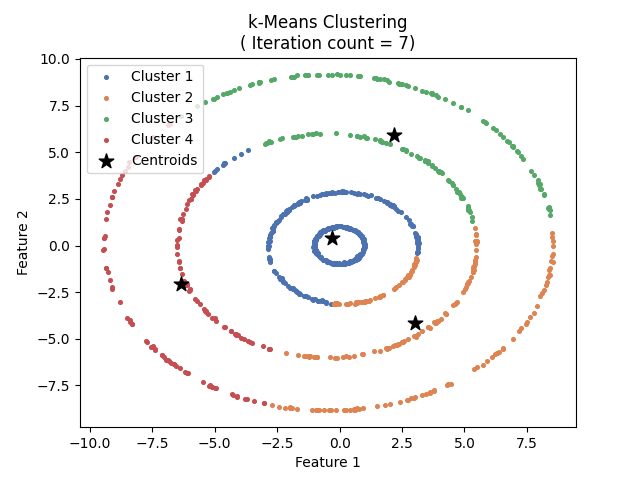
\includegraphics[width=.32\textwidth]{Q2b4_K4_3.png}
\textbf{Figure 18 :} Run 3: no of clusters = 4\\

\hangindent=0.0cm 

\hangindent=4.5cm 
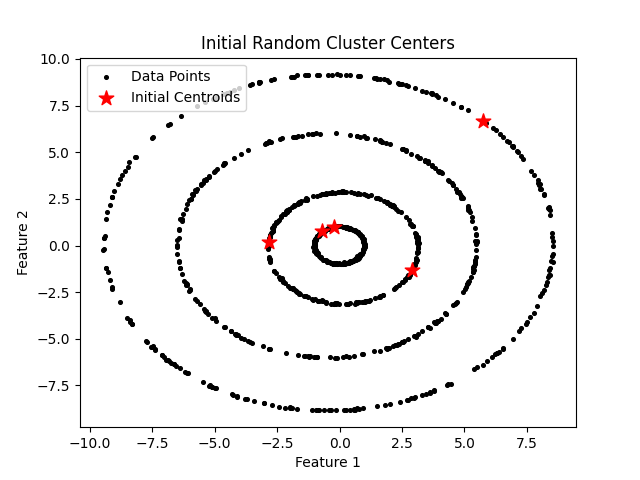
\includegraphics[width=.32\textwidth]{Q2b5_K4_1.png}\hfill
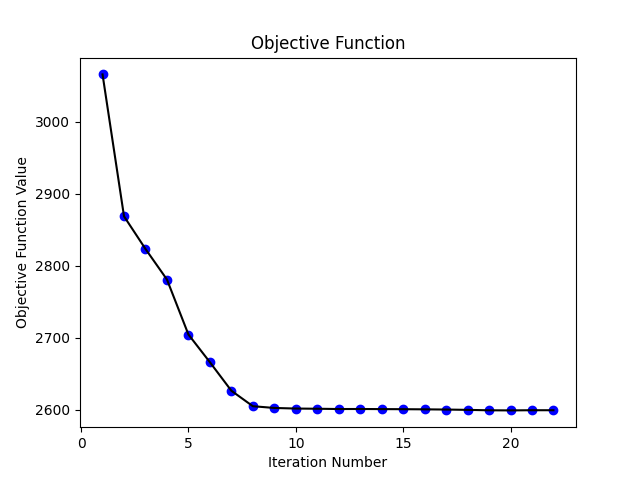
\includegraphics[width=.32\textwidth]{Q2b5_K4_2.png}\hfill
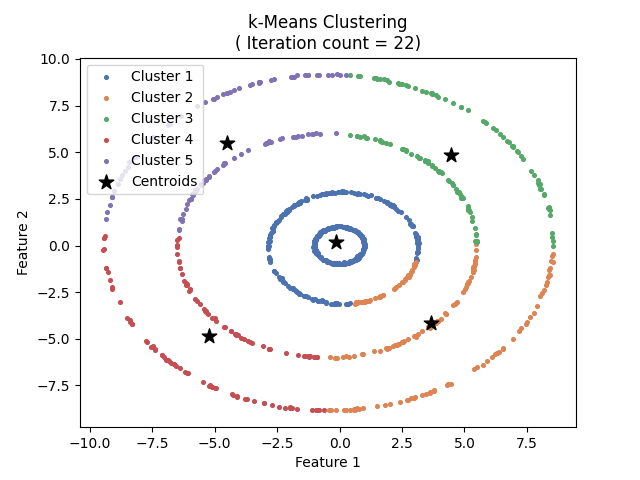
\includegraphics[width=.32\textwidth]{Q2b5_K4_3.png}
\textbf{Figure 18 :} Run 4: no of clusters = 5\\

\hangindent=0.0cm 

\end{solution}

\part Run the spectral clustering algorithm (spectral relaxation of K-means using Kernel- PCA) k = 4. Choose an appropriate kernel for this data-set and plot the clusters
obtained in different colors. Explain your choice of kernel based on the output
you obtain.
\begin{solution}\\


\hangindent=4.5cm 
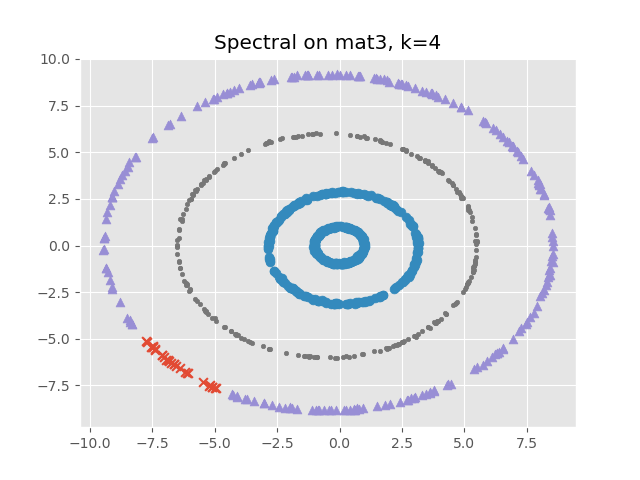
\includegraphics[width=.80\textwidth]{Q2c_1.png}\hfill

\hangindent=4.5cm 
\textbf{Figure 19 :} Spectral Clustering , K=4\\

\hangindent=0.0cm 
Used the Radical Basic function as function approximation. 
The idea behind the self tuning spectral clustering is determine the optimal number of clusters and also the similarity metric σi used in the computation of the affinity matrix. We can achieve using the RBF.


\hangindent=0.0cm 
\end{solution}

\part Instead of using the method suggested by spectral clustering to map eigenvectors to cluster assignments, use the following method: Assign data point $i$ to cluster $l$ whenever
\[ l = arg \max_{j=1,...k} v^j_i\]
where $v^j 	\in {R}^n$ is the eigenvector of the Kernel matrix associated with the $j^th$ largest eigenvalue. How does this mapping perform for this dataset?. Explain
your insights.
\begin{solution}\\
It is failed to converge it self or might not able to output good solution.

\end{solution}
\end{parts}

\end{questions}
\end{document} \documentclass[solution,addpoints,12pt]{exam}
\usepackage{amsmath}
\usepackage{amsthm}
\usepackage{amssymb}
\usepackage{tikz}
\usepackage{animate}
\usepackage{hyperref}

\newtheorem{theorem}{Theorem}
\newtheorem{lemma}[theorem]{Lemma}

\newenvironment{Solution}{\begin{EnvFullwidth}\begin{solution}}{\end{solution}\end{EnvFullwidth}}

\printanswers
%\unframedsolutions
\pagestyle{headandfoot}

%%%%%%%%%%%%%%%%%%%%%%%%%%%%%%%%%%%%%%%%%%%%%%%%%%%%%%
%%%%%%%%%%%%%%%%%%% INSTRUCTIONS %%%%%%%%%%%%%%%%%%%%%
% * Fill in your name and roll number below

% * Answer in place (after each question)

% * Use \begin{solution} and \end{solution} to typeset
%   your answers.
%%%%%%%%%%%%%%%%%%%%%%%%%%%%%%%%%%%%%%%%%%%%%%%%%%%%%%
%%%%%%%%%%%%%%%%%%%%%%%%%%%%%%%%%%%%%%%%%%%%%%%%%%%%%%

% Fill in the details below
\def\studentName{\textbf{Name: Hanumantappa Budihal}}
\def\studentRoll{\textbf{Roll No: cs21m022}}
\firstpageheader{CS5691 (PRML)-Assignment1 }{}{\studentName,\studentRoll}
\firstpageheadrule

\newcommand{\brac}[1]{\left[ #1 \right]}
\newcommand{\curly}[1]{\left\{ #1 \right\}}
\newcommand{\paren}[1]{\left( #1 \right)}
\newcommand{\card}[1]{\left\lvert #1 \right\rvert}

\begin{document}

\noindent \textbf{CS5691}: Pattern recognition and machine learning
Assignment 1
\\
\begin{flushright}
\textbf{Name and Signature}\\
Hanumantappa Budihal\\
\hangindent=3.5cm \includegraphics[width=4cm]{Sign.PNG} 
\end{flushright}
\begin{questions}

\question {\textbf{Question 1 :}}

\begin{parts}
\part  Write a piece of code to run the PCA algorithm on this data-set. How much of
the variance in the data-set is explained by each of the principal components?
\begin{solution}\\
The code for PCA is in the attached code file named question \textbf{Q1.py.}\\

Variance along first principal component is  \textbf{54.178025\%} of total variance.

Variance along the second principal component  \textbf{is 45.821975\%} of total variance.\\

The total of variance observed by data along principal components is =\\ \textbf{31.621519151774}

\end{solution}
\part Study the effect of running PCA without centering the data-set. What are your
observations? Does Centering help?
\begin{solution}
By running the PCA on the given data without centering, the result obtained are as follows:\\

Total of variance along principal components     : \textbf{31.621519151774983}

Variance along first principal component         : \textbf{54.178025\%}

Variance along second principal component        :\textbf{ 45.821975\%}\\

Form (a) and (b) we can see that the percentage of variance observed by each of principal components are the same in case of centered and non-centered data.
\\

Hence , we can say that for given data centering does not help, below figure is shown for the centered data\\

\hangindent=5.5cm 
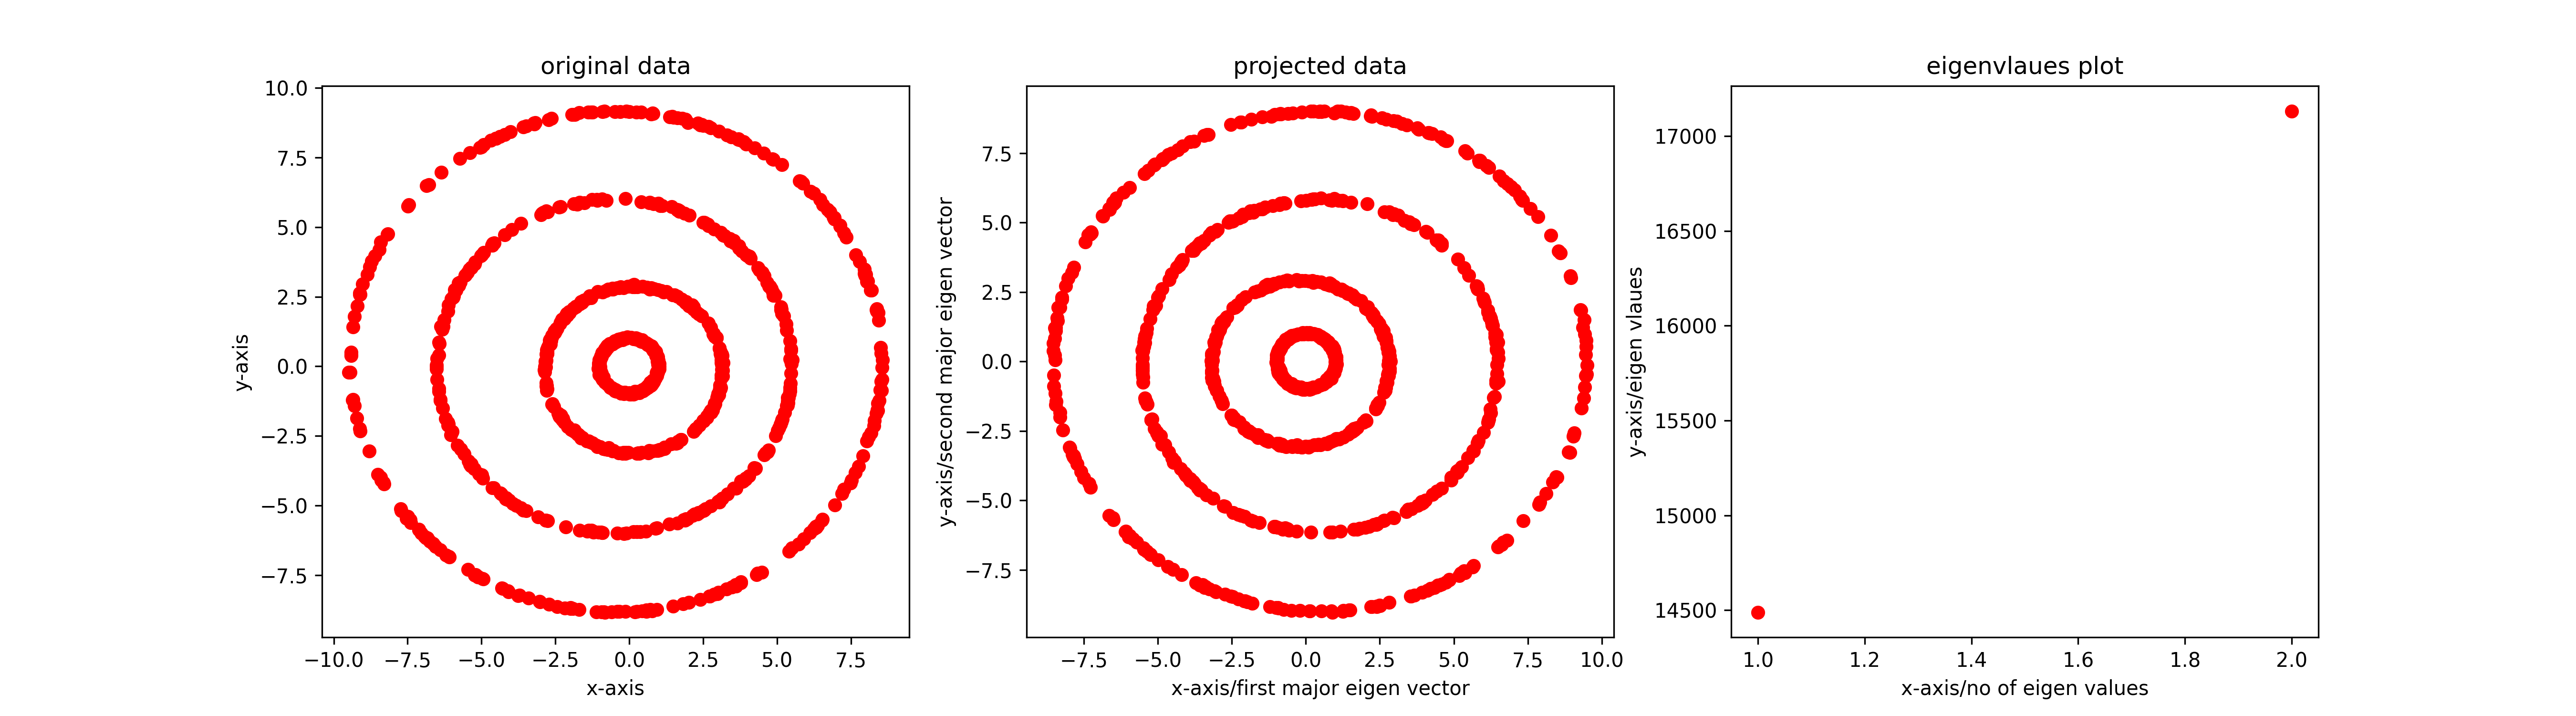
\includegraphics[width=15cm,height=5cm]{A.png}
\textbf{Figure1 :}  Result of centered data\\

Below figure shows the results for non-centered data	

\hangindent=5.5cm 
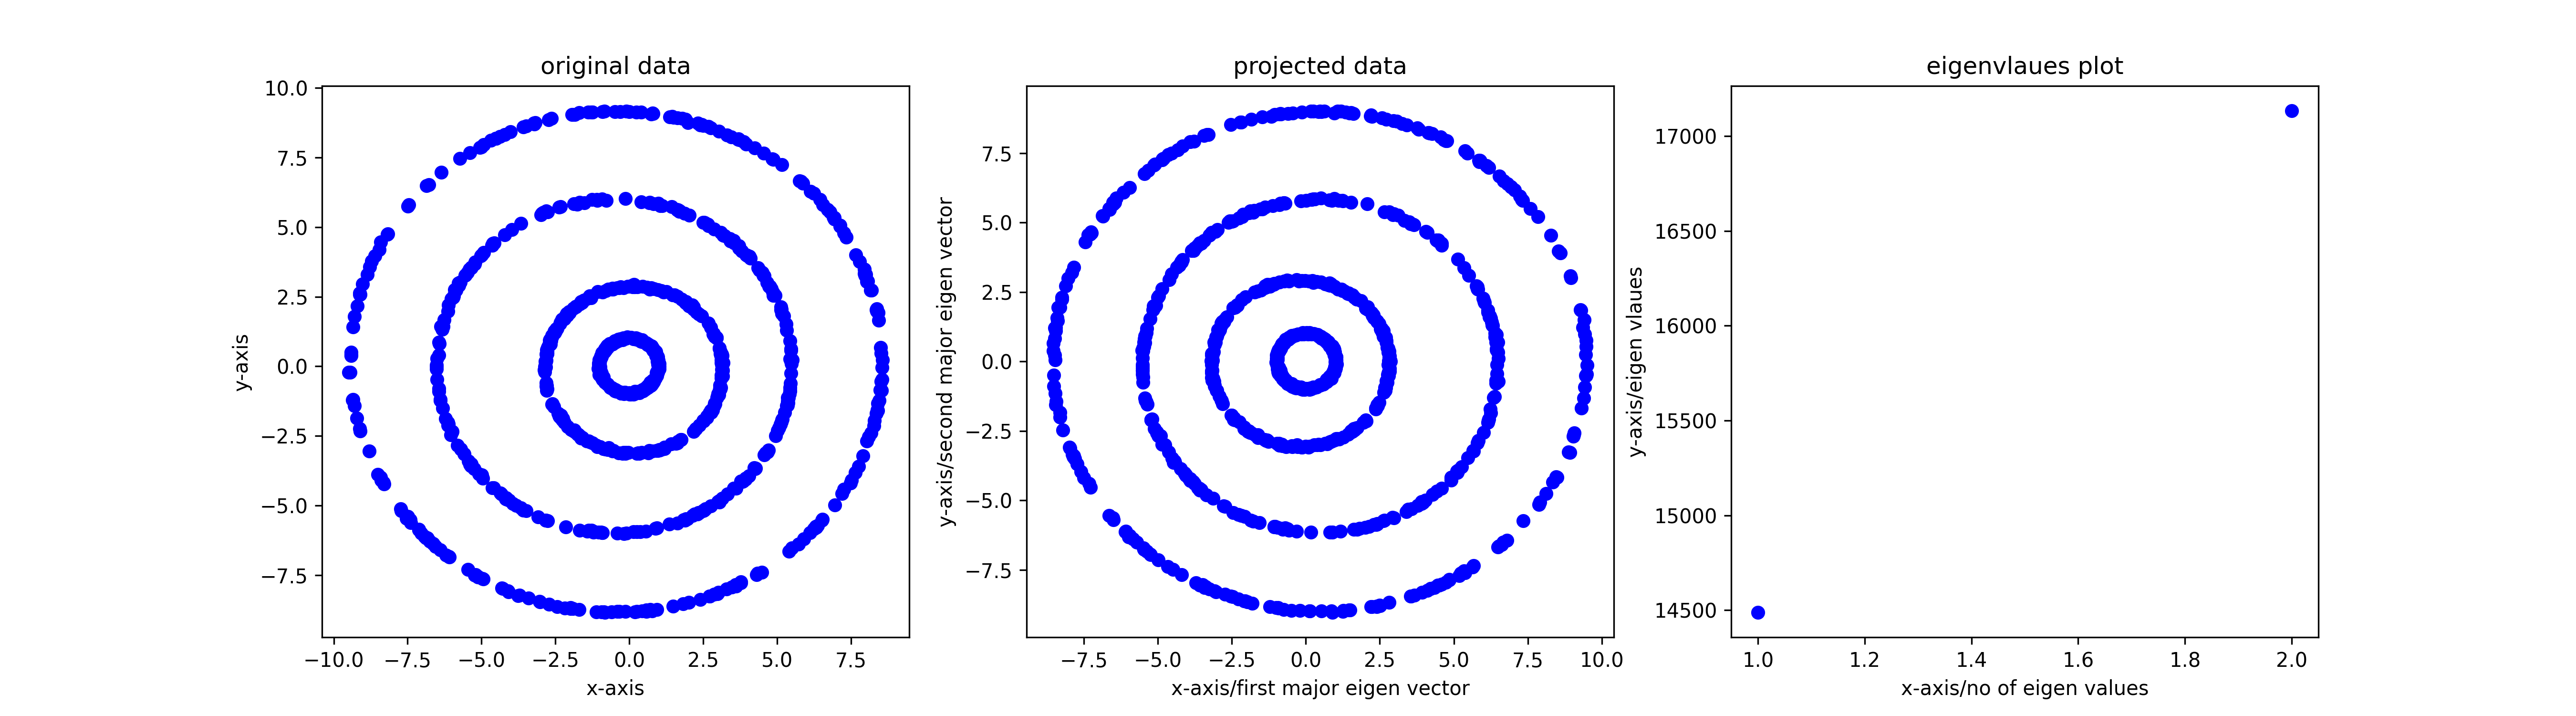
\includegraphics[width=15cm,height=5cm]{cA.png}
\textbf{Figure2 :}  Result of non centered data\\

\hangindent=0.0cm 
As the given data is already centered so centering does not plays any role here.

From figure it is clear that PCA is not able to do any helpful transformation on data, because, after projecting data onto eigen space we are obtaining the same data.\\

Also we are having the initial total variance of given data = total variance of projected data. as the data is circular around the origin, any pair of perpendicular vectors can become principal components directions.\\

\end{solution}
\part Write a piece of code to implement the Kernel PCA algorithm on this dataset.
Use the following kernels :

A. $k(x,y) = (1+x^Ty)^d$ for d = {2,3}

B. $k(x,y)= exp \frac{-(x-y)^T(x-y)}{2\sigma^2}$ for $\sigma={0.1,0.2,....,1}$

Plot the projection of each point in the dataset onto the top-2 components for
each kernel. Use one plot for each kernel and in the case of (B), use a different
plot for each value of $\sigma$
\begin{solution}
\textbf{Plots for kernel $k(x,y) = (1+x^Ty)^d$ are shown below}\\ 

\hangindent=5.5cm 
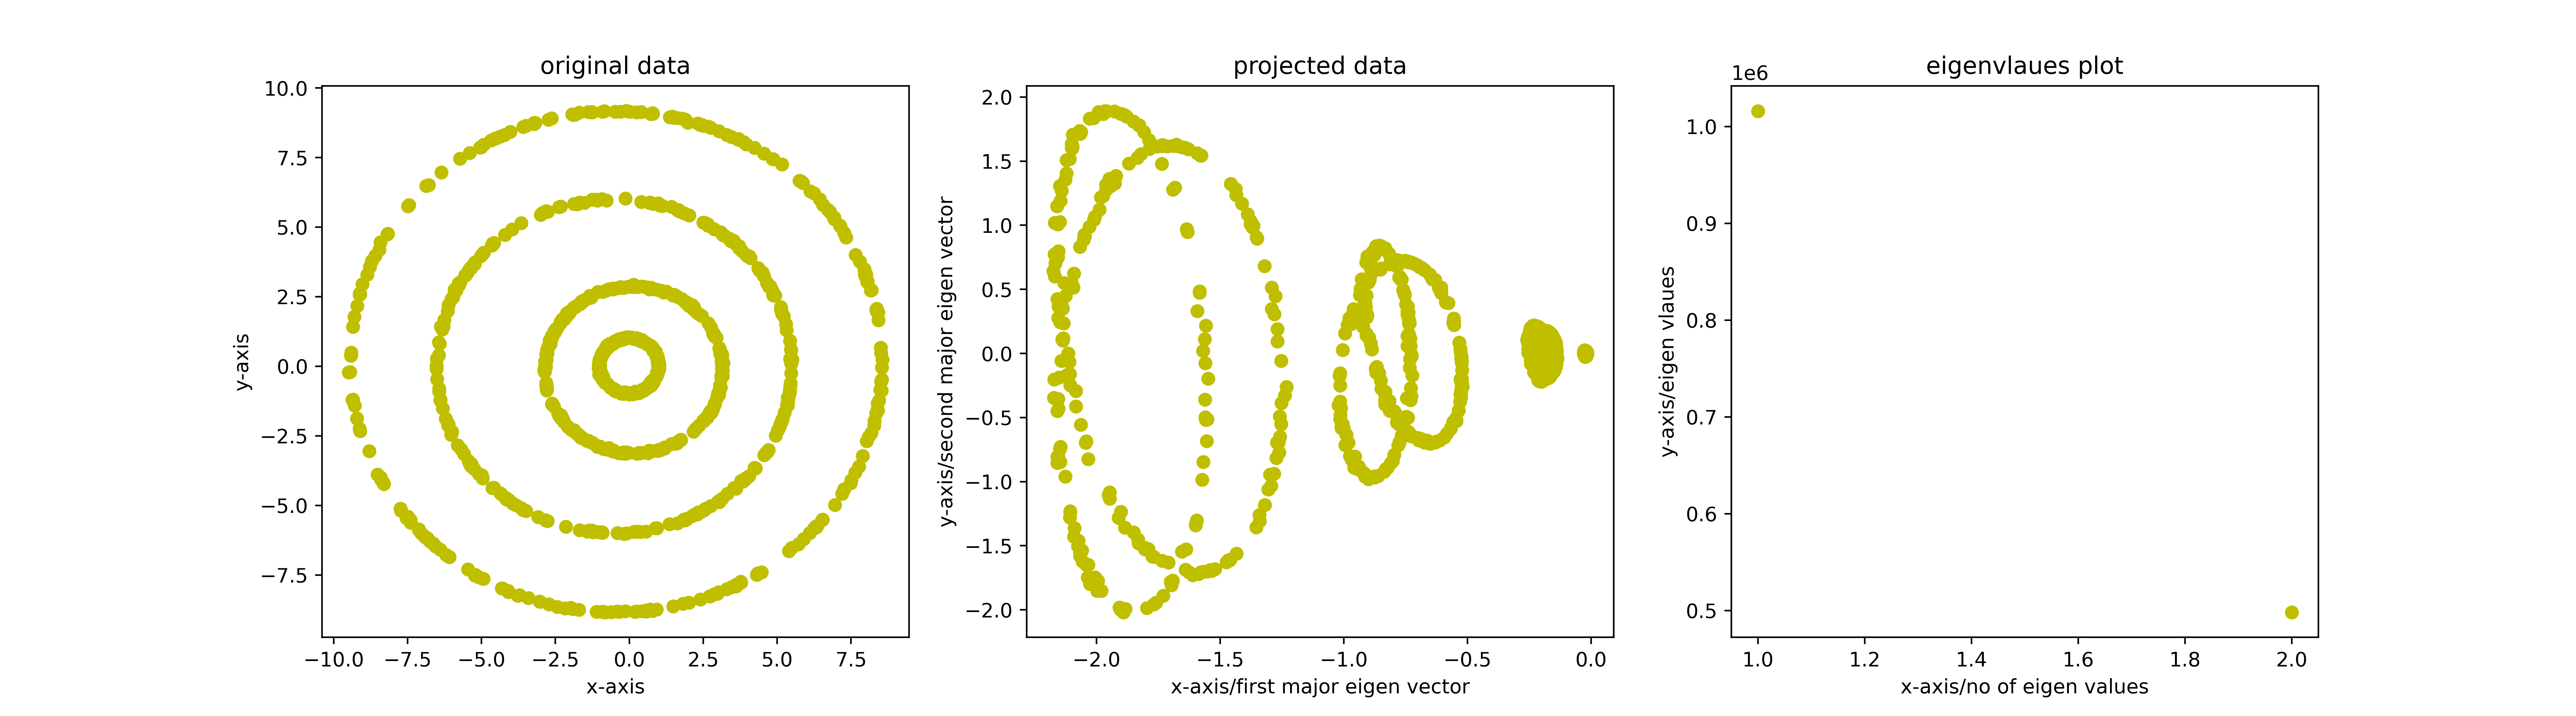
\includegraphics[width=15cm,height=5cm]{2.png}
\textbf{Figure 3 :} for d=2 \\

\hangindent=0.0cm 

\hangindent=5.5cm 
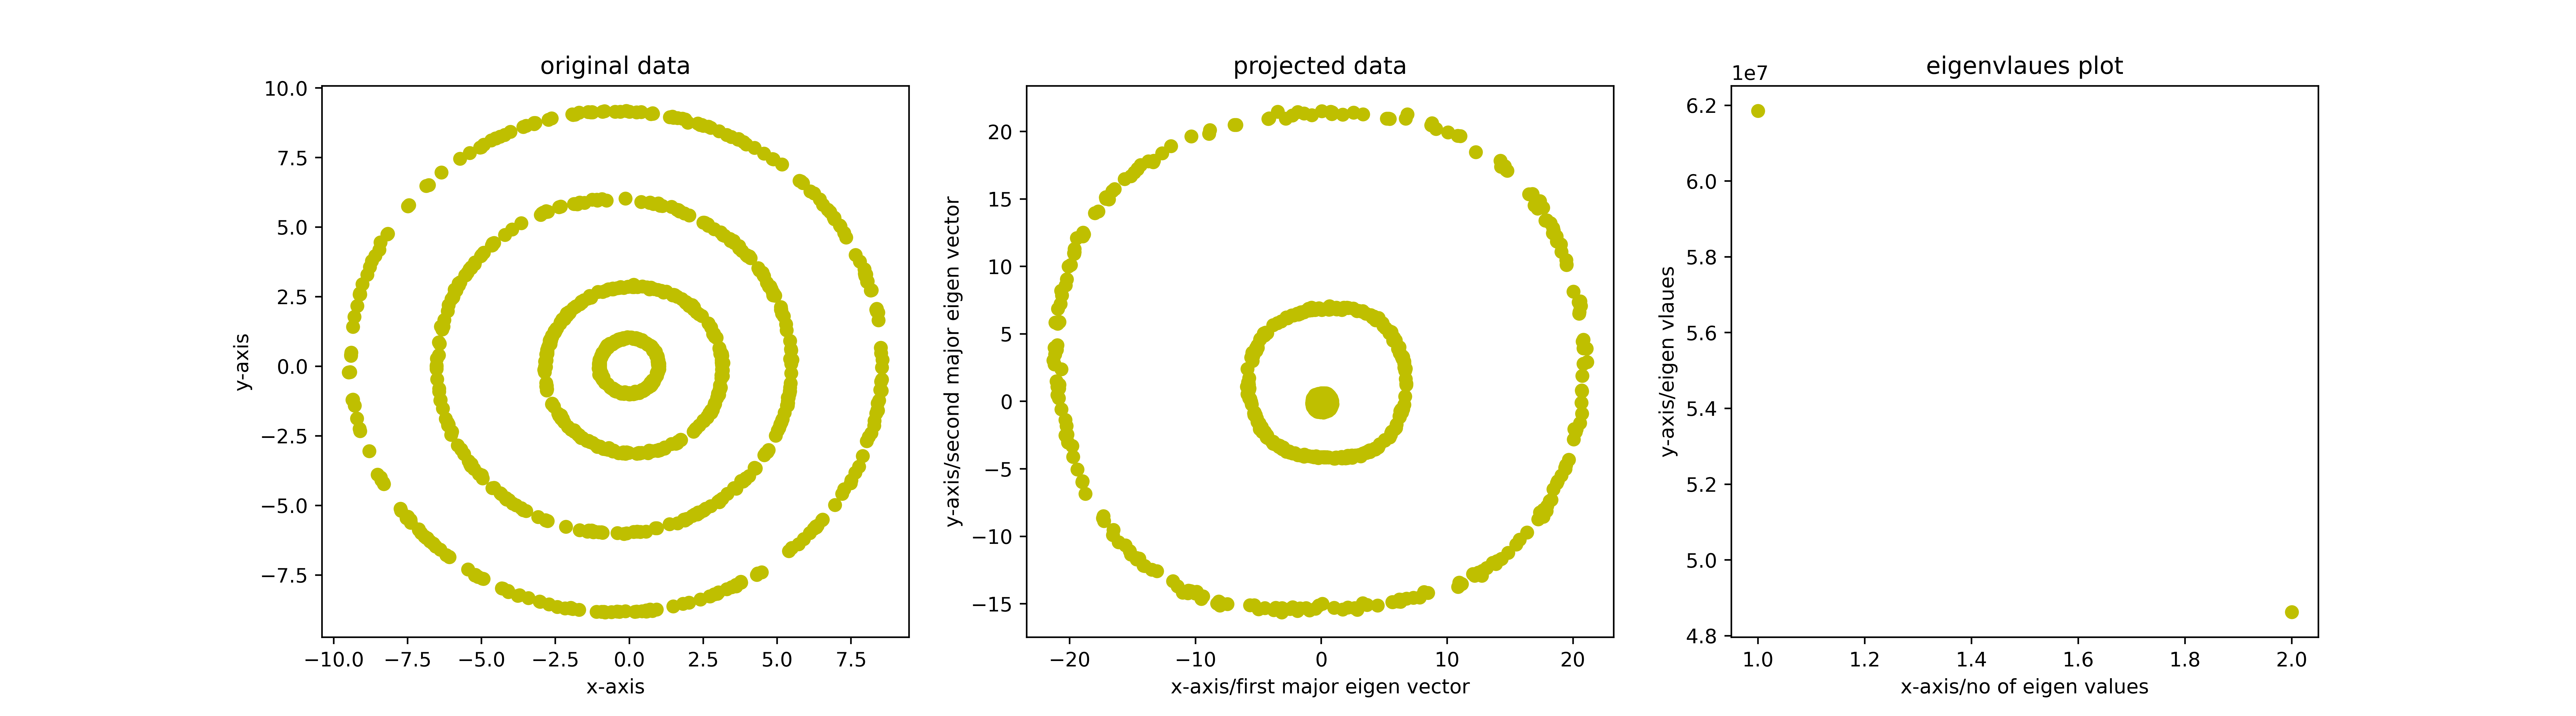
\includegraphics[width=15cm,height=5cm]{3.png}
\textbf{Figure 4 :} for d=3 \\

\hangindent=0.0cm 

\textbf{Plots for kernel $k(x,y) = (1+x^Ty)^d$ are shown below}\\ 

\hangindent=5.5cm 
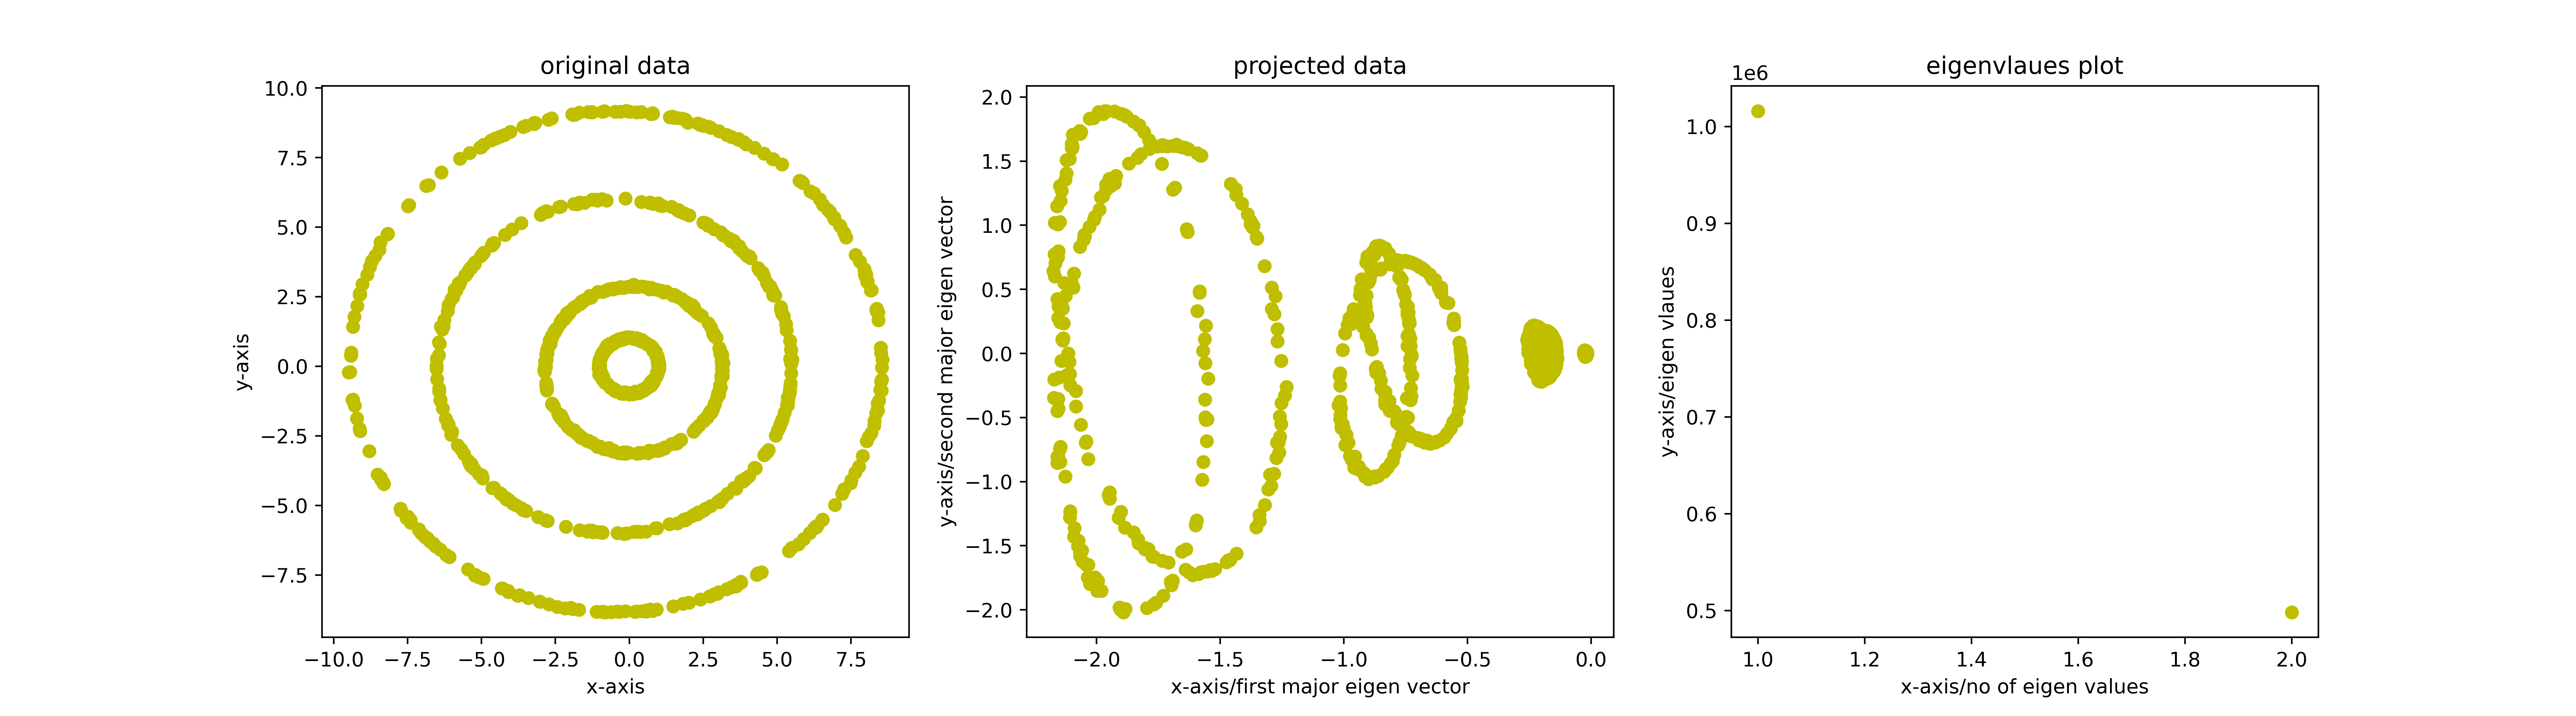
\includegraphics[width=15cm,height=5cm]{2.png}
\textbf{Figure 5:} for $\alpha$=0.1\\

\hangindent=0.0cm 

\hangindent=5.5cm 
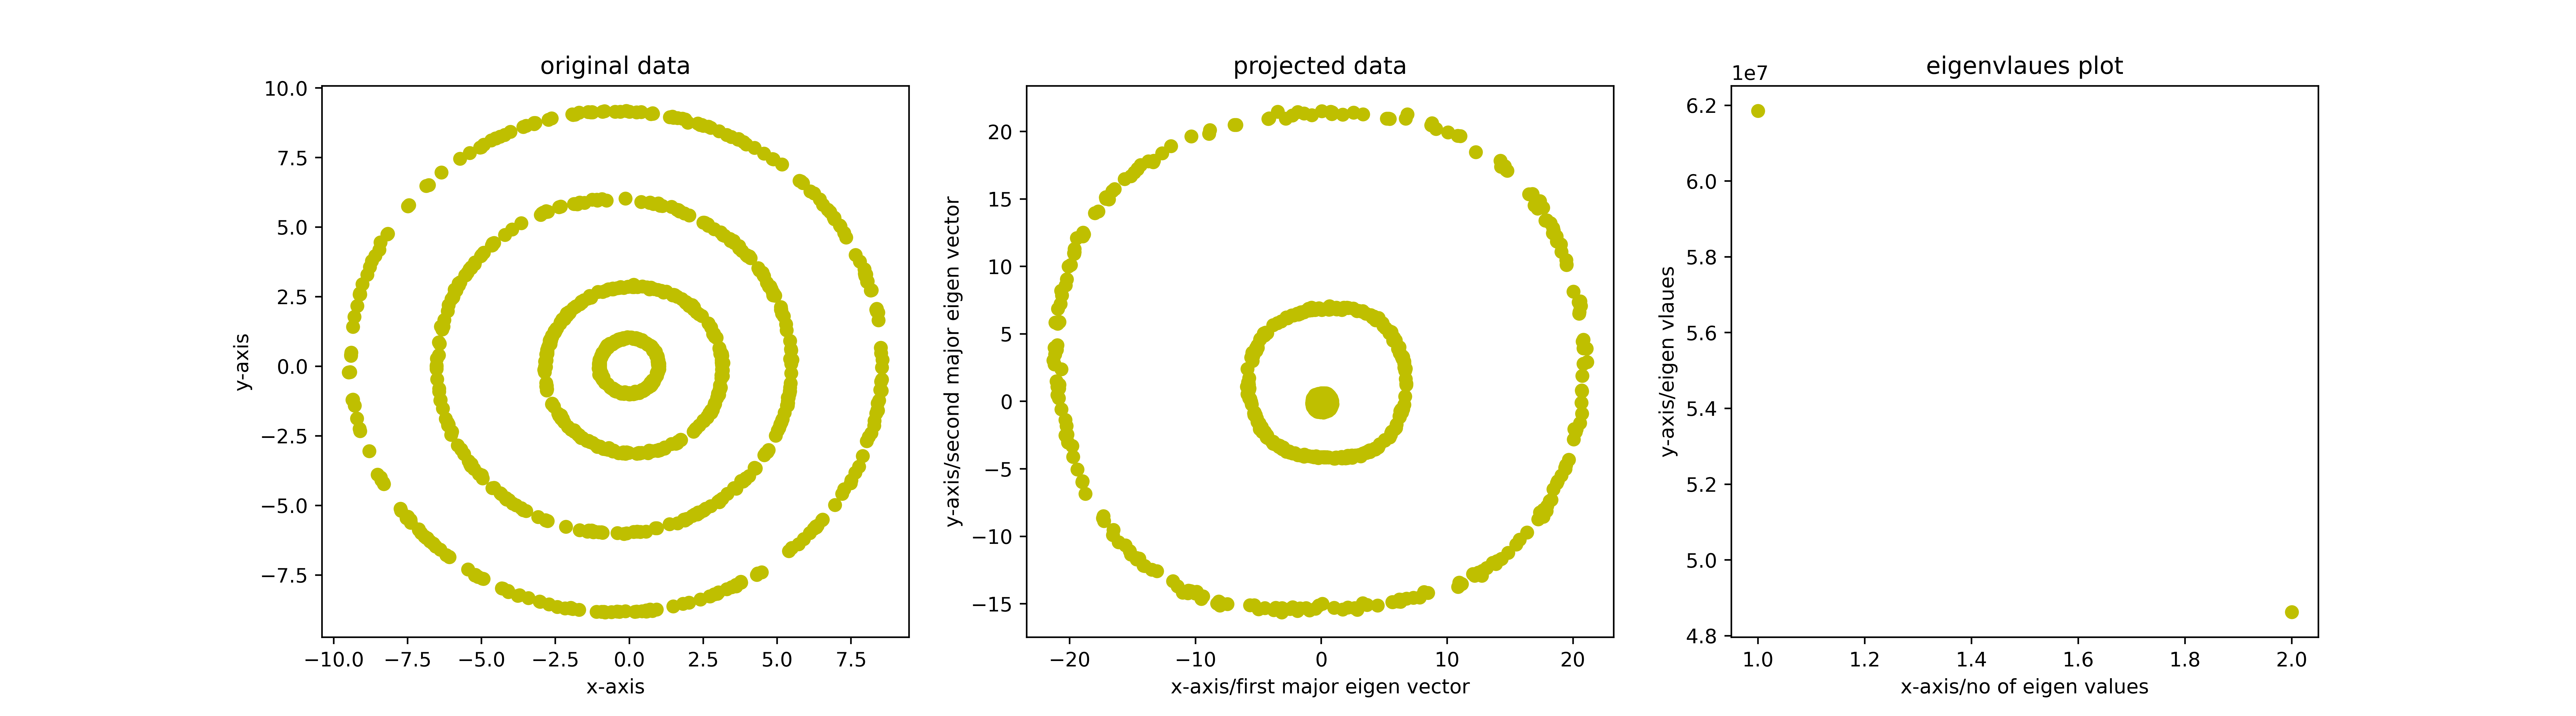
\includegraphics[width=15cm,height=5cm]{3.png}
\textbf{Figure 6 :} for $\alpha$=0.2 \\

\hangindent=0.0cm 

\hangindent=5.5cm 
\includegraphics[width=15cm,height=5cm]{3k2.png}
\textbf{Figure 7 :} for $\alpha$=0.3 \\

\hangindent=0.0cm 

\hangindent=5.5cm 
\includegraphics[width=15cm,height=5cm]{4k2.png}
\textbf{Figure 8 :} for $\alpha$=0.4 \\

\hangindent=0.0cm 

\hangindent=5.5cm 
\includegraphics[width=15cm,height=5cm]{5k2.png}
\textbf{Figure 9 :} for $\alpha$=0.5 \\

\hangindent=0.0cm 
 
\hangindent=5.5cm 
\includegraphics[width=15cm,height=5cm]{6k2.png}
\textbf{Figure 10 :} for $\alpha$=0.6 \\

\hangindent=0.0cm 

\hangindent=5.5cm 
\includegraphics[width=15cm,height=5cm]{7k2.png}
\textbf{Figure 11 :} for $\alpha$=0.7 \\

\hangindent=0.0cm 

\hangindent=5.5cm 
\includegraphics[width=15cm,height=5cm]{8k2.png}
\textbf{Figure 12 :} for $\alpha$=0.8 \\

\hangindent=0.0cm 

\hangindent=5.5cm 
\includegraphics[width=15cm,height=5cm]{9k2.png}
\textbf{Figure 13 :} for $\alpha$=0.9 \\

\hangindent=0.0cm 

\hangindent=5.5cm 
\includegraphics[width=15cm,height=5cm]{10k2.png}
\textbf{Figure 14 :} for $\alpha$=1.0 \\

\hangindent=0.0cm 

\end{solution}
\part Which Kernel do you think is best suited for this dataset and why?
\begin{solution} The gaussian kernel is best suited for this dataset with σ as 1,because it is capturing maximum variance among all other values of σ. The polynomial kernel is not able to properly de-correlate the data; it can be seen from figure 3 and figure 4 as compared to the gaussian kernel.

\end{solution}

\end{parts}

\question .

\begin{parts}
\part Write a piece of code to run the algorithm studied in class for the K-means
problem with k = 4 . 5 different random initialization and plot the error
function w.r.t iterations in each case. In each case, plot the clusters obtained in
different colors.
\begin{solution}

\hangindent=5.5cm 
\includegraphics[width=.33\textwidth]{Q2a1_K4_1.png}\hfill
\includegraphics[width=.33\textwidth]{Q2a1_K4_2.png}\hfill
\includegraphics[width=.33\textwidth]{Q2a1_K4_3.png}
\textbf{Figure 15 :} Run 1 : no of clusters = 4\\

\hangindent=0.0cm 

\hangindent=5.5cm 
\includegraphics[width=.33\textwidth]{Q2a2_K4_1.png}\hfill
\includegraphics[width=.33\textwidth]{Q2a2_K4_2.png}\hfill
\includegraphics[width=.33\textwidth]{Q2a2_K4_3.png}
\textbf{Figure 16 :} Run 2 : no of clusters = 4\\

\hangindent=0.0cm 

\hangindent=5.5cm 
\includegraphics[width=.33\textwidth]{Q2a3_K4_1.png}\hfill
\includegraphics[width=.33\textwidth]{Q2a3_K4_2.png}\hfill
\includegraphics[width=.33\textwidth]{Q2a3_K4_3.png}
\textbf{Figure 17 :} Run 3 : no of clusters = 4\\

\hangindent=0.0cm 

\hangindent=5.5cm 
\includegraphics[width=.33\textwidth]{Q2a4_K4_1.png}\hfill
\includegraphics[width=.33\textwidth]{Q2a4_K4_2.png}\hfill
\includegraphics[width=.33\textwidth]{Q2a4_K4_3.png}
\textbf{Figure 17 :} Run 4 : no of clusters = 4\\

\hangindent=0.0cm 

\hangindent=5.5cm 
\includegraphics[width=.33\textwidth]{Q2a5_K4_1.png}\hfill
\includegraphics[width=.33\textwidth]{Q2a5_K4_2.png}\hfill
\includegraphics[width=.33\textwidth]{Q2a5_K4_3.png}
\textbf{Figure 17 :} Run  5: no of clusters = 4\\

\hangindent=0.0cm 

\end{solution}

\part Fix a random initialization. For $K = {2,3,4,5}$, obtain cluster centers according
to K-means algorithm using the fixed initialization. For each value of K, plot the
Voronoi regions associated to each cluster center. (You can assume the minimum
and maximum value in the data-set to be the range for each component of R2).\\
\begin{solution} Fixed a random initialization and  $K = {2,3,4,5}$,\\

\hangindent=5.5cm 
\includegraphics[width=.32\textwidth]{Q2b2_K4_1.png}\hfill
\includegraphics[width=.32\textwidth]{Q2b2_K4_2.png}\hfill
\includegraphics[width=.32\textwidth]{Q2b2_K4_3.png}
\textbf{Figure 18 :} Run  1: no of clusters = 2\\

\hangindent=0.0cm 

\hangindent=4.5cm 
\includegraphics[width=.32\textwidth]{Q2b3_K4_1.png}\hfill
\includegraphics[width=.32\textwidth]{Q2b3_K4_2.png}\hfill
\includegraphics[width=.32\textwidth]{Q2b3_K4_3.png}
\textbf{Figure 18 :} Run 2: no of clusters = 3\\

\hangindent=0.0cm 

\hangindent=4.5cm 
\includegraphics[width=.32\textwidth]{Q2b4_K4_1.png}\hfill
\includegraphics[width=.32\textwidth]{Q2b4_K4_2.png}\hfill
\includegraphics[width=.32\textwidth]{Q2b4_K4_3.png}
\textbf{Figure 18 :} Run 3: no of clusters = 4\\

\hangindent=0.0cm 

\hangindent=4.5cm 
\includegraphics[width=.32\textwidth]{Q2b5_K4_1.png}\hfill
\includegraphics[width=.32\textwidth]{Q2b5_K4_2.png}\hfill
\includegraphics[width=.32\textwidth]{Q2b5_K4_3.png}
\textbf{Figure 18 :} Run 4: no of clusters = 5\\

\hangindent=0.0cm 

\end{solution}

\part Run the spectral clustering algorithm (spectral relaxation of K-means using Kernel- PCA) k = 4. Choose an appropriate kernel for this data-set and plot the clusters
obtained in different colors. Explain your choice of kernel based on the output
you obtain.
\begin{solution}\\


\hangindent=4.5cm 
\includegraphics[width=.80\textwidth]{Q2c_1.png}\hfill

\hangindent=4.5cm 
\textbf{Figure 19 :} Spectral Clustering , K=4\\

\hangindent=0.0cm 
Used the Radical Basic function as function approximation. 
The idea behind the self tuning spectral clustering is determine the optimal number of clusters and also the similarity metric σi used in the computation of the affinity matrix. We can achieve using the RBF.


\hangindent=0.0cm 
\end{solution}

\part Instead of using the method suggested by spectral clustering to map eigenvectors to cluster assignments, use the following method: Assign data point $i$ to cluster $l$ whenever
\[ l = arg \max_{j=1,...k} v^j_i\]
where $v^j 	\in {R}^n$ is the eigenvector of the Kernel matrix associated with the $j^th$ largest eigenvalue. How does this mapping perform for this dataset?. Explain
your insights.
\begin{solution}\\
It is failed to converge it self or might not able to output good solution.

\end{solution}
\end{parts}

\end{questions}
\end{document} 